% %%%%%%%%%%%%%%%%%%%%%%%%%%%%%%%%%%%%%%%%%%%%%%%%%%%%%%%%%%%%%%%%%%%%%%%%%%
% AGUtmpl.tex: this template file is for articles formatted with LaTeX2e,
% Modified July 2014
%
% This template includes commands and instructions
% given in the order necessary to produce a final output that will
% satisfy AGU requirements.
%
% PLEASE DO NOT USE YOUR OWN MACROS
% DO NOT USE \newcommand, \renewcommand, or \def.
%
% FOR FIGURES, DO NOT USE \psfrag or \subfigure.
%
%%%%%%%%%%%%%%%%%%%%%%%%%%%%%%%%%%%%%%%%%%%%%%%%%%%%%%%%%%%%%%%%%%%%%%%%%%%%
%
% All questions should be e-mailed to latex@agu.org.
%
%%%%%%%%%%%%%%%%%%%%%%%%%%%%%%%%%%%%%%%%%%%%%%%%%%%%%%%%%%%%%%%%%%%%%%%%%%%%
%
% Step 1: Set the \documentclass
%
% There are two options for article format: two column (default)
% and draft.
%
% PLEASE USE THE DRAFT OPTION TO SUBMIT YOUR PAPERS.
% The draft option produces double spaced output.
%
% Choose the journal abbreviation for the journal you are
% submitting to:

% jgrga JOURNAL OF GEOPHYSICAL RESEARCH
% gbc   GLOBAL BIOCHEMICAL CYCLES
% grl   GEOPHYSICAL RESEARCH LETTERS
% pal   PALEOCEANOGRAPHY
% ras   RADIO SCIENCE
% rog   REVIEWS OF GEOPHYSICS
% tec   TECTONICS
% wrr   WATER RESOURCES RESEARCH
% gc    GEOCHEMISTRY, GEOPHYSICS, GEOSYSTEMS
% sw    SPACE WEATHER
% ms    JAMES
% ef    EARTH'S FUTURE
% ea    EARTH AND SPACE SCIENCE
%
%
%
% (If you are submitting to a journal other than jgrga,
% substitute the initials of the journal for "jgrga" below.)

\documentclass[draft,jgrga]{agutex2015}
% To create numbered lines:

% If you don't already have lineno.sty, you can download it from
% http://www.ctan.org/tex-archive/macros/latex/contrib/ednotes/
% (or search the internet for lineno.sty ctan), available at TeX Archive Network (CTAN).
% Take care that you always use the latest version.

% To activate the commands, uncomment \usepackage{lineno}
% and \linenumbers*[1]command, below:

 \usepackage{lineno}
 \linenumbers*[1]
%  To add line numbers to lines with equations:
%  \begin{linenomath*}
%  \begin{equation}
%  \end{equation}
%  \end{linenomath*}
%%%%%%%%%%%%%%%%%%%%%%%%%%%%%%%%%%%%%%%%%%%%%%%%%%%%%%%%%%%%%%%%%%%%%%%%%
% Figures and Tables
%
%
% DO NOT USE \psfrag or \subfigure commands.
%
%
%  Uncomment the following command to include .eps files
%  (comment out this line for draft format):
%%  \usepackage[dvips]{graphicx}
\usepackage[dvipdfmx]{graphicx}
\usepackage{mediabb}
%\usepackage{here}
%
%  Uncomment the following command to allow illustrations to print
%   when using Draft:
  \setkeys{Gin}{draft=false}
%
% Substitute one of the following for [dvips] above
% if you are using a different driver program and want to
% proof your illustrations on your machine:
%
% [xdvi], [dvipdf], [dvipsone], [dviwindo], [emtex], [dviwin],
% [pctexps],  [pctexwin],  [pctexhp],  [pctex32], [truetex], [tcidvi],
% [oztex], [textures]
%
% See how to enter figures and tables at the end of the article, after
% references.
%
%% ------------------------------------------------------------------------ %%
%
%  ENTER PREAMBLE
%
%% ------------------------------------------------------------------------ %%

% Author names in capital letters:
\authorrunninghead{USUI ET AL.}

% Shorter version of title entered in capital letters:
%\titlerunninghead{ELECTRON DYNAMICS IN MINI-MAGNETOSPHERE}
\titlerunninghead{BOUNDARY CURRENT IN MINI-MAGNETOSPHERE}

%Corresponding author mailing address and e-mail address:
\authoraddr{Corresponding author: H. Usui,
Graduate School of System Informatics, 
Kobe University, 1-1 Rokkoudai-cho, Nada-ku, Kobe 657-8501, JAPAN
(h-usui@port.kobe-u.ac.jp)}

\begin{document}

%% ------------------------------------------------------------------------ %%
%
%  TITLE
%
%% ------------------------------------------------------------------------ %%


\title{
Boundary layer current in the  
mini-magnetosphere above a lunar magnetic anomaly
%%Electron dynamics in the %boundary layer current of a
}
%

%% ------------------------------------------------------------------------ %%
%
%  AUTHORS AND AFFILIATIONS
%
%% ------------------------------------------------------------------------ %%


%Use \author{\altaffilmark{}} and \altaffiltext{}

% \altaffilmark will produce footnote;
% matching \altaffiltext will appear at bottom of page.

 \authors{
Hideyuki Usui,\altaffilmark{1}
 Yohei Miyake,\altaffilmark{2}
 Masaki Nishino\altaffilmark{3} 
 Takuma Matsubara,\altaffilmark{1}, and 
 Joseph Wang\altaffilmark{4}}

% \authors{A. B. Smith,\altaffilmark{1}
% Eric Brown,\altaffilmark{1,2} Rick Williams,\altaffilmark{3}
% John B. McDougall\altaffilmark{4}, and S. Visconti\altaffilmark{5}}

\altaffiltext{1}{
Graduate School of System Informatics,
Kobe University, Kobe, Hyogo, Japan
}

\altaffiltext{2}{
Education Center for Computational Science and Engineering, 
Kobe University, Kobe, Hyogo, Japan
}

\altaffiltext{3}{
Institute for Space-Earth Environment Research, Nagoya University, 
Nagoya, Aichi, Japan
}

\altaffiltext{4}{
Department of Astraunautical Engineering, The University of Southern California,
Los Angeles, California, USA.
}

%% ------------------------------------------------------------------------ %%
%
%  KEYPOINTS
%
%% ------------------------------------------------------------------------ %%
% Key points are 1 to 3 points that the author provides,
% that are 100 characters or less, that are ultimately published
% with the article.
%% for example:
% \keypoints{\item Here is the first keypoint. what happens if it is a
% long keypoint, like this one. We want to see this wrap please.
% \item This is the second.
% \item And here is the third keypoint
% }

\keypoints{
%%\item Boundary layer current in a mini-magnetosphere has a structure of electron turn-around flux
\item The electron current dominates the 
boundary layer of a mini-magnetosphere above a lunar magnetic anomaly.
\item The electron boundary current shows 
two symmetric structures in which the convection reverses direction
with respect to the magnetic equator.
\item Electrons in the innermost boundary layer obtain 
maximum velocity due to the acceleration by the electric field due to charge separation.
%%\item The width of the boundary layer current approximately equals
%%the radius of the local cyclotron motion of electrons
}

%% Keypoints will print underneath the abstract.
%% ------------------------------------------------------------------------ %%
%
%  ABSTRACT
%
%% ------------------------------------------------------------------------ %%

% >> Do NOT include any \begin...\end commands within
% >> the body of the abstract.

\begin{abstract}
We consider a three-dimensional electromagnetic
particle-in-cell simulation of
the boundary layer current in a mini-magnetosphere
created by the interaction between a magnetized plasma flow,
which models the typical solar wind, and
a small-scale magnetic dipole, which represents
the Reiner Gamma magnetic anomaly on the lunar surface.
The size of this magnetic anomaly
(measured as the distance from the dipole center
to the position where the pressure of the local magnetic field
equals the dynamic pressure of the solar wind)
is one quarter that of the Larmor radius of the solar wind ions.
In spite of the weak magnetization of the ions,
a mini-magnetosphere is formed above the magnetic anomaly.
In the boundary layer of the mini-magnetosphere,
the electron current is dominant.
Due to the intense electric field induced by charge separation,
electrons entering the boundary layer undergo 
$\mbox{\boldmath $E$} \times \mbox{\boldmath $B$}$ drift.
In each hemisphere, the electron boundary current due to the drift shows a 
structure where the convection reverses; these structures are symmetric with respect to the magnetic equator.
Detailed analysis of the electron cyclotron motion
shows that electrons at the edge of the inner boundary layer
obtain maximum velocity by the electric field acceleration
due to the charge separation, 
not due to the drift of the electron's guiding center. 
The maximum electron velocity is approximately eight times 
that of the upstream plasma. 
The width of the boundary layer current becomes approximately 
equal to the radius of the local electron cyclotron. 
\end{abstract}

%% ------------------------------------------------------------------------ %%
%
%  BEGIN ARTICLE
%
%% ------------------------------------------------------------------------ %%

% The body of the article must start with a \begin{article} command
%
% \end{article} must follow the references section, before the figures
%  and tables.

\begin{article}

%% ------------------------------------------------------------------------ %%
%
%  TEXT
%
%% ------------------------------------------------------------------------ %%

\section{Introduction}
The lunar plasma environment has been investigated 
intensively by recent spacecraft,  such as
KAGUYA \citep[e.g.,][]{Saito2008,Saito2010,Saito2012} and
Chandrayaan-1 \citep[e.g.,][]{Barabash2009,Bhardwaj2010}.
In addition to macroscopic plasma structures,
such as the wake structure formed in the downstream region,
small-scale perturbations of plasma distribution and fields have been
 observed in the dayside region,
mostly over the crustal magnetic anomalies found on the lunar surface.
The KAGUYA spacecraft observed
more than $10 \%$ of the solar wind protons reflected at an altitude of approximately 100 km
over the magnetic anomalies [\cite{Saito2010}].
Chandrayaan-1 determined that the deflection of the solar wind protons was highly efficient (greater than $ 10 \%$) [\cite{Lue2011}], and it
also observed backstreaming hydrogen atoms over the magnetic anomalies [\cite{Wieser2010}].
It was also found that
plasma wave activities were enhanced over the magnetic anomalies
\citep[e.g.,][]{Halekas2006a,Hashimoto2010}.
These observations suggest that the plasma and field disturbances over
the magnetic anomalies are caused by interactions of the solar wind with the local magnetic field.
Unlike the Earth's magnetosphere, %however, 
the dipole moment of
the lunar magnetic anomalies is very weak, and
the resulting dipole field region is much smaller than the characteristic spatial scales
of the solar wind, such as the inertial length and Larmor radius $r_\mathrm{iL}$ of the ions.



% 2015/1011 modified - L definition -
%
When the direction of the solar wind is orthogonal to the dipole moment 
$\mbox{\boldmath $M$}$,
we can characterize the size of the magnetic dipole immersed 
in the solar wind by a distance $L$ from the dipole center to 
the upstream position at which the pressure of the local magnetic field 
equals the dynamic pressure of the solar wind at the magnetic equator. 
Since for the plasma, we do not consider the finite Larmor radius effect,  
We use the magnetohydrodynamics (MHD) approximation for $L$.
To derive $L$, 
We use the following formulation for a dipole magnetic field in free space: 
\begin{linenomath}
 \begin{equation}
  \mbox{\boldmath $B$}
  =
 \frac{\mu_{\mathrm{0}}}{4\pi} 
 \Bigl(
 \frac{3(\mbox{\boldmath $M$} \cdot \mbox{\boldmath $r$}) \mbox{\boldmath $r$} }{r^{5}}
 -
 \frac{\mbox{\boldmath $M$}}{r^{3}}
  \Bigr)
 \label{eqn:B}
 \end{equation}
\end{linenomath}
where $\mbox{\boldmath $r$}$ is the position vector with respect to the dipole center, and $\mu_{\mathrm{0}}$ is the permeability in a vacuum, respectively.
When $\mbox{\boldmath $M$}$ is set to be perpendicular to the solar wind, 
we can obtain the intensity of the dipole field $|B|$
from Equation (\ref{eqn:B}) as a function of the intensity of the magnetic moment $|M|$ and
the upstream position $x$ from the dipole center along the sunward direction:
\begin{linenomath}
 \begin{equation}
 |B| = 
 \frac{\mu_{\mathrm{0}} |M| }{4\pi x^3} 
 \label{eqn:B_at_x}
 \end{equation}
\end{linenomath}
By setting $x=L$ in the above equation, 
we can calculate $|B|$ for the location at which  
the magnetic pressure equals the dynamic pressure of the solar wind. 
Then, $L$ is obtained as follows (as shown in \cite{Ashida2014}):
\begin{linenomath}
 \begin{equation}
  L =
  \Bigl(
  \frac{\mu_{\mathrm{0}} M^{2}}
  {16 \pi^{2} m_{\mathrm{i}} n_{\mathrm{0}} v_{\mathrm{flow}}^{2}}
  \Bigr)^\frac{1}{6}
 \label{eqn:L}
 \end{equation}
\end{linenomath}
% 
where $n_{\mathrm{0}}$ and $v_{\mathrm{flow}}$ are the density and velocity of the plasma flow, respectively, and $m_{\mathrm{i}}$ is the ion mass.  
For lunar magnetic anomalies,
$L$ is less than or equal to 100 km, which is smaller than $r_\mathrm{iL}$.
In such a situation,
the protons are almost unmagnetized, and their dynamics are not affected significantly 
by the local field of magnetic anomalies.
However, as stated above,
a variety of related phenomena, such as the reflection and deflection of ions, have been observed.
Above magnetic anomalies, the mechanism underlying the ion dynamics is thought to be due to the interactions of the solar wind with those anomalies.
%%%Hide, is this what you want to say here??

The interactions between a plasma flow and a small-scale magnetic dipole 
have been examined in various situations.
The mesoscale is the region in which $L$ is less than or comparable to $r_\mathrm{iL}$
but larger than the electron Larmor radius $r_\mathrm{eL}$.
In a feasibility study of a magnetosail proposed for a interplanetary flight system, two-dimensional
particle-in-cell (PIC) plasma simulations were used to examine
the interactions of the solar wind with the mesoscale magnetic dipole that was artificially created by the
superconducting coil on the spacecraft [\cite{Moritaka2012}].
That study showed the formation of a magnetosphere even in the mesoscale regime.
In interactions between the solar wind and a mesoscale magnetic dipole, it was found that at the magnetopause,
the electrons are magnetized, but the magnetization of the ions is reduced.
An electric field is induced in the dayside magnetosphere as charges are separated
due to the difference between the momentum of the electrons and that of the ions.
It was shown that the electric field induced at the magnetopause
can affect the dynamics of the incoming solar wind ions, and some of the ions can be reflected
back in the sunward direction.

A similar interaction takes place between the solar wind and lunar magnetic anomalies.
A mini-magnetosphere with a density cavity has been studied both by
 spacecraft observations and by numerical simulations
\citep[e.g.,][]{Harnett2000,Harnett2003,Halekas2008b,Bamford2012}.
The plasma responses to the induced electric field have also been examined
by conducting particle simulations
\citep[e.g.,][]{Harnett2002,Kallio2012,Poppe2012a,Deca2014,Deca2015}.
Laboratory experiments of plasma interactions
with a small-scale magnetic dipole
were also conducted, and the electric field 
induced by the interaction
between a plasma flow and the local magnetic field has been examined
\citep[e.g.,][]{Howes2015,Jarvinen2014,Wang2013,Bamford2012}.
%-- comment by referee2---
The interaction of the solar wind with a magnetic anomaly was also 
examined using a hybrid particle simulation that used  
an empirical model of the Gerasimovich magnetic anomaly, which was based 
on observations of the Lunar Prospector 
\citep{Fatemi2015}.
%-----

As has been pointed out in many previous studies,
plasma kinetics, such as the finite Larmor radius effect, should be included when modeling
the interactions between the solar wind and magnetic anomalies
because $L$ is almost the same as or smaller than $r_\mathrm{iL}$.
The electric field generated by
charge separation at the magnetopause affects 
the dynamics of the solar wind ions and 
causes their reflection and deflection. %  affected and some of them are reflected.
Meanwhile, the solar wind electrons are magnetized in the mini-magnetosphere.
Hence, the boundary layer current is mainly due to the electron flux.
It has been reported that the motion of electrons in the boundary layer 
is primarily 
$\mbox{\boldmath $E$} \times \mbox{\boldmath $B$}$ drift.
The velocity distribution function of electrons at different locations above
the magnetic anomaly were examined in \cite{Deca2015}.
However, the details of the three-dimensional structure of the boundary layer current,
which is dominated by the electron flux, have not been determined.
% 2016/10/6 
In addition, 
the microscopic dynamics of electrons in the boundary layer has not been
examined, nor has the electron cyclotron motion (ECM).
%

In this study,
we use three-dimensional electromagnetic particle-in-cell simulations to investigate the spatial structure of the boundary layer current 
in a mini-magnetosphere formed above a lunar magnetic anomaly.
We focus on the electron dynamics in the boundary layer.
In Section II, we describe the simulation method, model, and parameters used in this study.
To examine the interactions between the solar wind and the Reiner Gamma magnetic anomaly, we used a magnetized plasma flow and a small-scale magnetic dipole; 
the plasma flow was parallel to the lunar surface, and the magnetic dipole was perpendicular to
the direction of plasma flow.
For the magnetic anomaly in our simulation, we let $r_\mathrm{iL} /L=4$.
In Section III, we show the spatial variation of the plasma density and the current density
by cutting different planes in the three-dimensional space obtained by the simulations.
In addition to the density profiles of the mini-magnetosphere created by the above magnetic anomaly, 
we also examine the three-dimensional structure of the boundary layer current.
In Section IV, we consider in detail the electron dynamics on the magnetic equator,
particularly at the innermost edge of the boundary layer of the mini-magnetosphere, 
where the electron density decreases to zero.
We summarize our results and present our conclusions in Section V.


\section{Simulation methods, model, and parameters}
This study is based on three-dimensional, full kinetic,
electromagnetic particle-in-cell (EM-PIC) simulations.
The basic numerical procedures used in the EM-PIC simulation are 
described in \cite{Birdsall1991}.  
In a PIC simulation, 
both ions and electrons are treated as particles in order to include
the kinetic effects of the plasma particles, 
such as the finite Larmor radius and the charge separation 
between the different species of particles. 
To trace the motions, 
the equation of motion is solved for individual particles of both species.
%the charge and velocity of all the particles are assigned 
%to each grid point to obtain the charge and current densities, respectively.
By using the updated velocity and position of the particles, the charge conservation method
is used to calculate the current density at each spatial grid point; this method is based on the continuity equation 
for the charged particles [\cite{Villasenor1992}].
To calculate the evolution of electromagnetic fields in the simulation domain,
Maxwell's equations are solved at each time step
by using the finite-difference time-domain method.
In Maxwell's equations, plasma dynamics are taken into account through
the current density obtained at each grid point.

Table 1 shows typical solar wind parameters,
which we used to model the upstream plasma, and the parameters we used for the Reiner Gamma magnetic anomaly.
As reported in \cite{kurata2005}, 
the Reiner Gamma magnetic anomaly is typical of those found on the lunar surface; it
is modeled as two magnetic dipoles, the southwest dipole (SW) and the northeast dipole (NE).
In this study, 
we focus on SW, which has a dipole moment that is slightly
inclined from the horizontal plane.
Because it is located at a low latitude,
we can assume that the magnetic dipole moment is almost parallel to the lunar surface
and that it is perpendicular to the sunward direction. 

%When L/riL = 1, the ratio of the electron plasma frequency to the cyclotron frequency, 
%$\omega_pe/\Omega_pe$, was set to be 250 at a distance L from the dipole center. 

%% - Table 1-
\begin{table}[h]
\caption{Parameters of the solar wind and the magnetic dipole of the Reiner Gamma anomaly}
%typical real parameters
\centering
 \begin{tabular}{p{16zw}ll}
 Parameters of the solar wind    &  Notations    &  Typical values \\  \hline           
% Mass ratio between ion and electron & $m_\mathrm{i}/m_\mathrm{e}$ & 1837 \\
 Density       & $n_\mathrm{e}$, $n_\mathrm{i}$  &  $3.5 \times 10^6 \mathrm{m^{-3}}$   \\ 
 Flow velocity & $v_\mathrm{flow}$               &  $400  \mathrm{km/s}  $              \\
 Mach number   & $M_\mathrm{A}$                  & 10.0 \\
 Beta          &  $\beta$                        & 0.96 \\
 Plasma temperature & $T_\mathrm{e}$, $T_\mathrm{i}$    &  $8.6$ eV \\
 Ratio between electron cyclotron frequency and plasma frequency & 
  $\Omega_\mathrm{ce}/\omega_\mathrm{pe}$ & $5.83 \times 10^{-3}$ \\ 
 Uniform magnetic field density &  $B_\mathrm{0}$   &   3.5 nT          \\ \hline 
  & & \\ 
 Parameters of Reiner Gamma    &  Notations    &  Typical values \\  \hline           
 Latitude and longitude   &  &  $7.5N, 58.4W$      \\   
 Inclination from the horizontal plane &      &   1.3 deg.         \\            
 Magnetic moment &  $ M $   &  $ 1.13 \times 10^{13} \mathrm{Am^2}$ \\
 Distance between the dipole center and the lunar surface & $L_\mathrm{surface}$ & 11 km \\ \hline
%% Balance point between the B-field energy and plasma dynamic pressure 
%% & $L$ &  32 km  from the dipole center  \\
%% Magnetic field density at $L$  & $B_\mathrm{L}$ & 34.3 nT  \\  \hline
 \end{tabular}
\end{table}
%%%%
%% - Table 2-
\begin{table}[h]
\caption{
Simulation parameters
}
\centering
 \begin{tabular}{p{16zw}ll}
 Parameters    &  Notations    &  Values \\  \hline           
 Mass ratio between ion and electron & $m_\mathrm{i}/m_\mathrm{e}$    & 100 \\
 Flow velocity                       & $v_\mathrm{flow} $  &  $0.05v_\mathrm{c}$ \\
 Mach number                         & $M_\mathrm{A}$ & 5.0 \\
 %Electron thermal velocity           & $v_\mathrm{the}$ &  $0.12v_\mathrm{c}$ \\
 Electron thermal velocity           & $v_\mathrm{the}$ &  $2.4v_\mathrm{flow}$ \\
 %Ion thermal velocity                & $v_\mathrm{thi}$ &  $ 0.012v_\mathrm{c}$ \\
 Ion thermal velocity                & $v_\mathrm{thi}$ &  $ 0.24v_\mathrm{flow}$ \\
 Ratio between electron cyclotron frequency and plasma frequency & 
  $\Omega_\mathrm{ce}/\omega_\mathrm{pe}$ & 0.1 \\  \hline

 Grid size                          &   $dr$  & $1.0\lambda_\mathrm{D}$  \\
 Time step                          &   $dt$  &  $0.285dr/v_\mathrm{c}$  \\
 Numbers of grids in the physical region  &  
 $N_x \times N_y \times N_z$        &  $192 \times 192 \times 192$  \\
 System dimensions                 &   
$l_x \times l_y \times l_z$ & $ 5.6L \times 5.6L \times 5.6L$  \\
 Depth of the dipole moment under the lunar surface  &   $L_\mathrm{dipole}$ 
 &  0.2$L$ \\  
 Ratio between the ion Larmor radius and $L$ & $ r_\mathrm{iL}/L$  & 4 \\ \hline
 \end{tabular}
\end{table}


%%%%%%%%%%%%%%%%%%%%%%%
%% - Figure 1-
\begin{figure}[t]
 \centering
 \noindent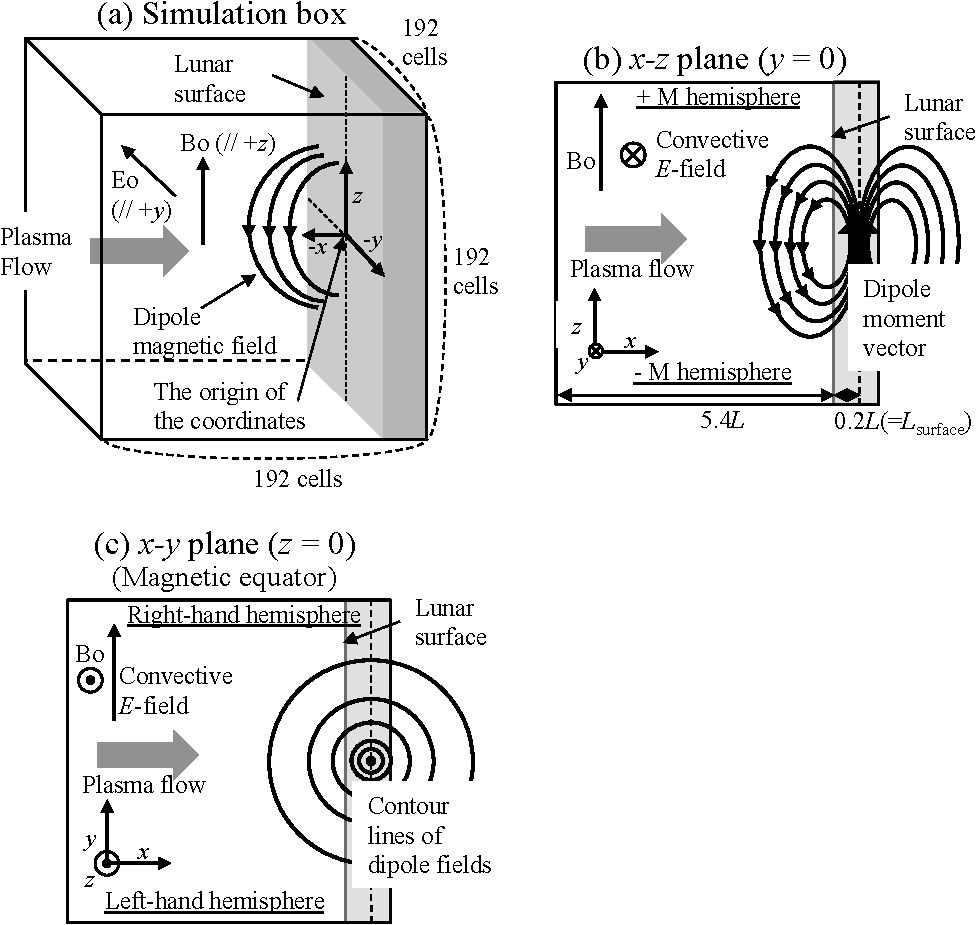
\includegraphics[]{./figures/Fig_1_bb-crop.pdf}
 \caption{(a) Three-dimensional simulation model, (b) $x-z$ plane, (c) $x-y$ plane}\label{fig:1}
\end{figure}

%%%%%%%%%%%%%%%%%%%%%%%

In Table 2, 
we list the simulation parameters used in this study. 
For the plasma flow representing the solar wind, 
instead of using the actual measured physical values listed in Table 1, 
we scaled them to reduce the calculation time. 
We set the mass ratio between ions and electrons in the plasma flow 
to be $ m_\mathrm{i}/ m_\mathrm{e}$ = 100, which allows us 
to clearly separate the dynamics of the two species of particles. 
We set the ratio of the speed of light $v_\mathrm{c}$ to 
$v_\mathrm{flow}$ to be 20, 
although the actual ratio is about 600. 
The plasma flow is isothermal, and 
the ratio of the electron thermal velocity 
$v_\mathrm{the}$ to $v_\mathrm{flow}$ is set to be 2.4, 
which is almost the same as the actual ratio for the solar wind electrons. 
The ion thermal velocity $v_\mathrm{thi}$ was set to $0.24v_\mathrm{flow}$.
We used a static magnetic field $B_0$ to represent the interplanetary magnetic field (IMF). 
The Alfv\'{e}nic Mach number $M_\mathrm{A}$, which is the ratio of $v_\mathrm{flow}$ to 
the Alfv\'{e}n velocity $v_\mathrm{A}$, was 5. 
For the solar wind, the beta value was set to unity, and the ratio of 
the electron cyclotron frequency to
the electron plasma frequency,
$\Omega_\mathrm{ce} / \omega_\mathrm{pe}$, 
was set to 0.1. 

Figure \ref{fig:1} shows the three-dimensional simulation model used in this study.
In the simulation domain, 
the grid size $dr$ corresponds to $\lambda_\mathrm{D}$, 
where $\lambda_\mathrm{D}$ denotes the Debye length in the plasma flow.
The time increment $dt$ was chosen to satisfy 
the Courant condition, $dr/dt > 1.73 v_\mathrm{c}$, in three dimensions. 
As shown in Panel (a) of Figure \ref{fig:1}, 
the simulation domain is a $192 \times 192 \times 192$ grid. 
%The length of each side of the domain is approximately $7.17L$. 
The length of each side of the domain is approximately $5.6L$. 
The electromagnetic perturbation propagating out of the simulation region
is attenuated in the absorbing region that encircles the outer boundary; the width of this region is 32 grid steps.
%The physical region surrounded by the field absorbing regions consists of 
%$192 \times 192 \times 192$ grids which corresponds to a cube $5.6L$ on each side. 
The lunar surface was $5.4L$ 
from the left boundary of the simulation region.
The coordinate origin was placed at the center of the lunar surface, 
as shown in Panel (a) of Figure \ref{fig:1}.

The upstream plasma was initialized uniformly with $v_\mathrm{flow}$,
and fresh plasma was continually injected from the left boundary of 
the simulation region along the positive $x$ direction,
which is the antisunward direction.
%The static magnetic field $B_0$ representing the interplanetary magnetic fields (IMF) 
%is also introduced in the simulation domain. 
We set $B_\mathrm{0}$ to be along the positive $z$ direction.
For the upstream plasma flow, a convective electric field $E_0$ was introduced along the positive $y$ direction 
so that condition $E_\mathrm{0} = -v_\mathrm{flow} \times B_\mathrm{0}$ 
was satisfied in the simulation domain. 
%%
%The plasma flow typically consists of $5.37 \times 10^8 $ 
%macroparticles in the simulation space. 
We did not consider particles crossing the lunar surface or other simulation boundaries. 
At the lunar surface, these particle velocities are counted as 
the electric current, and they are used to update the normal component
of the electric field. 
Note that the electric field at the lunar surface corresponds to the surface charge,
%% need to say something about charging ?
and for simplicity, we assume no photoelectron emissions from the surface. 

To show the configuration of the dipole field and each region 
in the simulation domain, 
we show two planes which are cut from the region shown in Figure \ref{fig:1} (a).
Figure \ref{fig:1} (b) shows the plane for which $y=0$.
On this plane, we set 
a magnetic moment 
$\mbox{\boldmath $M$}$ 
along the positive $z$ direction and
at a distance of $0.2L$ under the lunar surface.
The value of 
$\mbox{\boldmath $M$}$ 
is determined such that $r_\mathrm{iL}/L =4$ at a distance of $L$ from the dipole center.
%which corresponds to $0.8L$ altitude from the lunar surface. 
Using Equation (\ref{eqn:L}) and the parameters of the solar wind and the
Reiner Gamma anomaly shown in Table 1,
we obtain $L$ =32 km, and $r_\mathrm{iL}$ at $L$ is approximately 120 km. 
This implies that 
$r_\mathrm{iL}$ is approximately four times as large as $L$,
which nearly agrees with the simulation parameter $r_\mathrm{iL}/L =4$.
The dipole magnetic field and $B_\mathrm{0}$
are considered in the equation of motion 
when the velocity of each particle is updated. 
Maxwell's equations are used to determine the variation of the magnetic field.
Hereafter, the positive and negative $z$ regions will be referred to as the
+M and -M hemispheres, respectively, as shown in Figure \ref{fig:1} (b).

Figure \ref{fig:1} (c) shows the $z=0$ plane,
which corresponds to the magnetic equator.
For convenience, 
we define the regions of positive and negative $y$ as the R-hand and L-hand 
hemispheres, respectively.

We ran the simulation until the spatial variation of the plasma density reached a steady state. 
%The time period for each simulation was approximately equivalent 
%to several cyclotron periods of observing ions at a distance L from the dipole center.
%



\section{Simulation Results}

%% - Figure 2-
\begin{figure}[t]
\centering
\noindent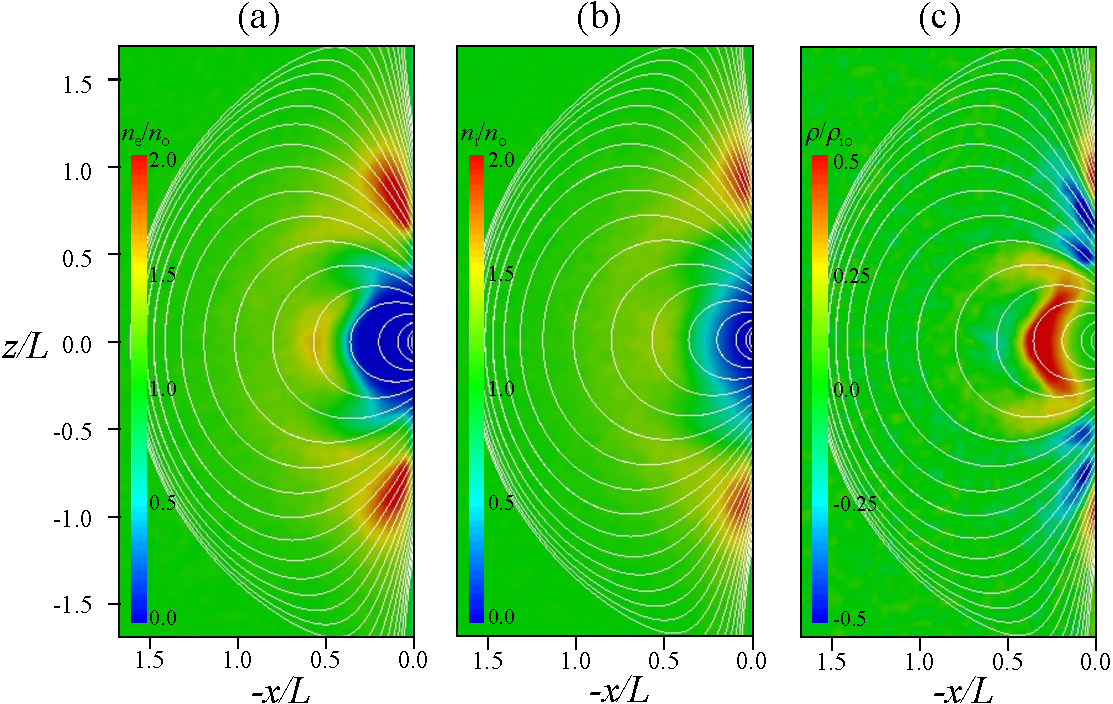
\includegraphics[width=15cm]{./figures/Fig_2_bb-crop.pdf}
\caption{Contour maps of (a) electron density, (b) ion density, and (c) charge density; 
obtained on the meridian plane $y/L=0$ at the steady state. The densities are normalized
to those in the unperturbed upstream plasma flow.}\label{fig:2}
\end{figure}

We examined the density profiles to see 
if a mini-magnetosphere was created by the interaction of
the plasma flow with the magnetic anomaly.
Figure \ref{fig:2} shows contour maps of the number density of electrons and ions  
and the charge density obtained at the steady state 
in the meridian plane, which includes $y/L = 0$. 
Note that $x/L=0$ represents the lunar surface, and 
the coordinate origin is located at the center of the lunar surface.
The plasma flows from the left boundary of 
the simulation domain and along the $x$ direction. 
The absolute value of $x$ coordinate is the altitude from the lunar surface.
In Figure \ref{fig:2}, as a reference,
we also show some of the field lines (in white) that originate from the dipole moment.
The intensities of the magnetic field at representative points along the line $y=z=0$
were $|B|/B_{\mathrm{0}} = 4.3$, $18$, and $70$ at $x/L=-1.0, -0.5$, and $-0.25$, respectively.
As shown in Figures \ref{fig:2} (a) and (b), 
a mini-magnetosphere with a plasma cavity is clearly 
created above the magnetic anomaly; this has been shown in 
previous studies
\citep[e.g.,][]{Harnett2000,Harnett2003,Halekas2008b,Bamford2012}.
The size of the mini-magnetosphere was less than $0.5L$.
Figure \ref{fig:2} (a) shows the electron density profile, and it can be seen that the boundary of the mini-magnetosphere is curved; this approximately corresponds to the dipole field structure, which is
shown in white.
It can also be seen that there is a sharp transition to 
the electron cavity region in the inner magnetosphere; for example,
the density transition occurred at $-x/L = 0.3$ 
along the line $z/L =0$.
We can also see that the density becomes relatively high 
in the high-latitude regions around
$|z|/L=0.8$ between the lunar surface and $-x/L=0.3$.
These regions correspond to the cusps at which the dipole fields converge to the poles.
In Figure \ref{fig:2} (b), which shows the ion density, 
we can confirm the formation of a mini-magnetosphere similar to the one shown 
in Figure \ref{fig:2} (a) for electrons.
However, 
the density gradient at the boundary of this mini-magnetosphere is 
not as high as that of the one for the electrons.
Because of their large inertia, some ions cross the line of the density transition seen in Figure \ref{fig:2} (a) and 
reach the inner magnetosphere. 
In addition, the mini-magnetosphere itself seems compressed toward the lunar surface.
The ion density becomes relatively high in the high-latitude regions, in which there is a 
high density of electrons. 
The spatial profiles of the mini-magnetospheres seen in Figures \ref{fig:2} (a) and (b) are similar;
however, because of the differences in the density profiles, as discussed above, 
there is a spatial variation in the charge density, as shown in Figure \ref{fig:2} (c). 
As can be seen, the ion density is highest near the magnetic equator and
within $|z|/L$ = 0.5 of the inner magnetosphere; this region is shown in red. 
However, near the lunar surface in both the hemispheres, in the high-latitude regions between $|z|/L \sim 0.5$ and 1.0, 
the electron density is relatively high; this region is shown in blue.
%%% Added 2016/1012
In the vicinity of the lunar surface $x/L=0$ and around $|z|/L=1.0$, 
we also see red regions, indicating that the ion density is high.
The density profiles in the vicinity of the lunar surface will be further discussed below.
%%%

% -- up here at the library in USC 2015/12/4 pm 4

%% - Figure 3-
\begin{figure}[t]
\centering
\noindent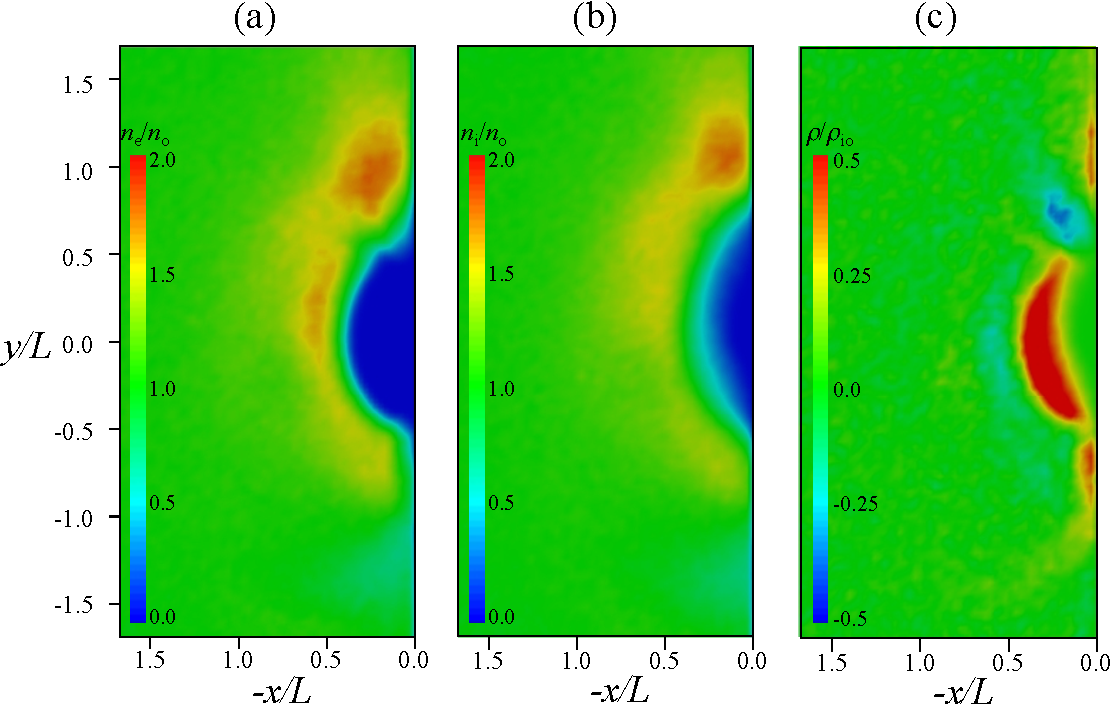
\includegraphics[width=15cm]{./figures/Fig_3_bb-crop.pdf}
\caption{
Contour maps of (a) electron density, (b) ion density, and (c) charge density; 
obtained at the magnetic equator $z/L=0$ at the steady state.
The densities are normalized to those in the unperturbed upstream plasma flow.
}
\label{fig:3}
\end{figure}

Figure \ref{fig:3} shows contour maps of the number density of 
electrons and ions and the charge density 
at the magnetic equator $z/L=0$, as in 
Figure \ref{fig:2}. 
One of the interesting features is that the density profiles 
in the boundary layer of the mini-magnetosphere
are asymmetric with respect to the line $y/L =0$.
As shown in Figures \ref{fig:3} (a) and (b), a high-density region is created 
for both electrons and ions in the upper region,
which corresponds to the R-hand hemisphere. 
The profile of the charge density shown in Figure \ref{fig:3} (c) is 
similar to that shown in Figure \ref{fig:2} (c). 
Since ions, which have a larger inertia than do electrons, can reach the inner magnetosphere, the region with a 
high density of ions (shown in red) is primarily located
along the inner boundary of the mini-magnetosphere. 
Like the profiles shown in Figures \ref{fig:3} (a) and (b), 
the charge density profile shown in Figure \ref{fig:3} (c) is asymmetric. 
In the R-hand hemisphere around $y/L = 0.5$ to 1.0, however, the region with a
high density of electrons (shown in blue) is close to the lunar surface. 
These plasma responses to a magnetic anomaly, 
including the formation of a mini-magnetosphere and 
the asymmetry of the plasma density, have been investigated 
in previous studies, and the charge separation at the boundary of the mini-magnetosphere has also been discussed
 \citep[e.g.,][]{Harnett2002,Kallio2012,Poppe2012a,Deca2014,Deca2015}.
These features were confirmed in our simulation results.

% 2016/1/17 upto here I read in a train to Kobe.

%% - Figure 4-
\begin{figure}[h]
\centering
\noindent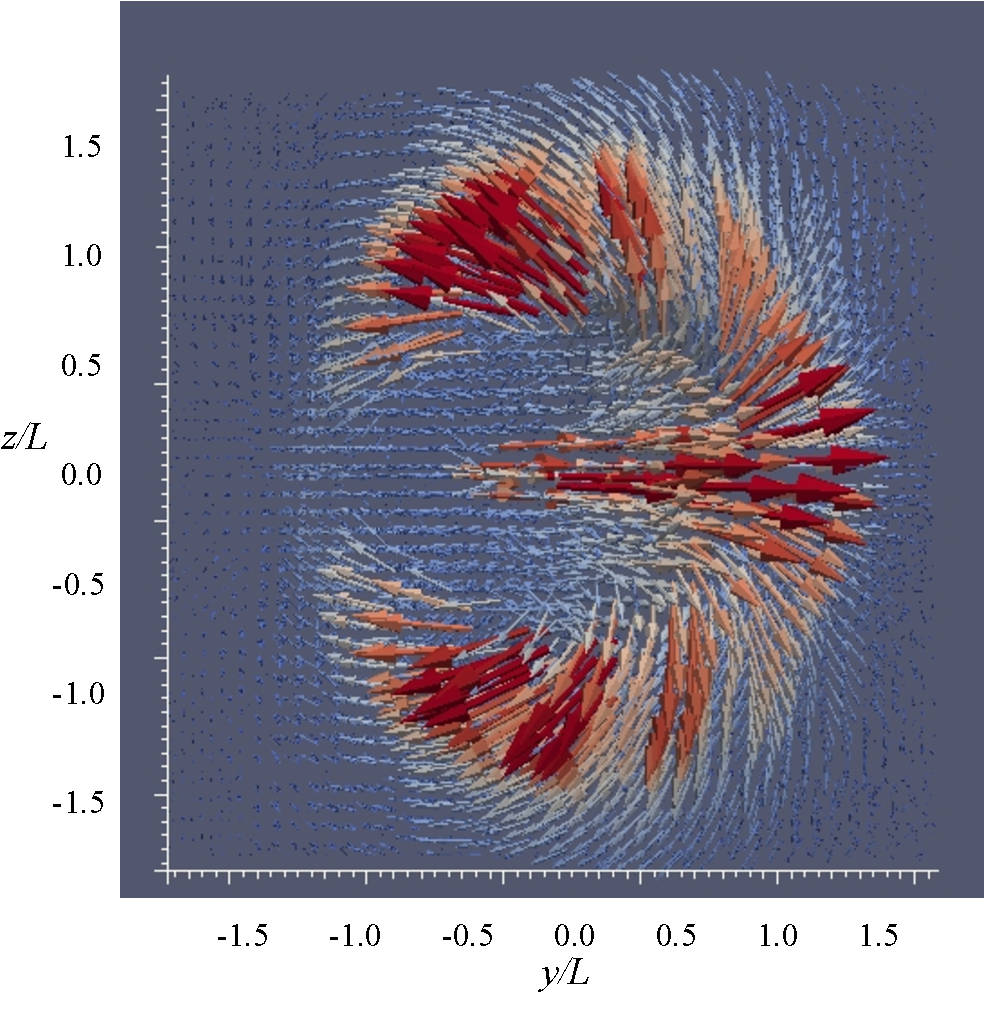
\includegraphics[width=12cm]{./figures/Fig_4_bb-crop.pdf}
\caption{
Vectors of current density in a three-dimensional region 
covered with $|y|/L=1.68$ and $|z|/L=1.68$ 
from the lunar surface up to a height of $x/L = -1.68$.
}
\label{fig:4}
\end{figure}

In this study, 
we are interested in the structure of the boundary layer current  
of the mini-magnetosphere.
In Figure \ref{fig:4}, 
we show the vectors of the current density in a three-dimensional region 
covered with $|y|/L=1.68$ and $|z|/L=1.68$, and 
from the lunar surface up to a height of $x/L = -1.68$.
%consisting of an area from $-1.68L$ to $1.68L$ in the $y-z$ plane
%with the altitude range from 0 to $1.68L$ from the lunar surface.
The plot is identical to an all-sky view of the current vectors
measured from the coordinate origin on the lunar surface. 
The current density values are normalized to 
the ion current density $J_\mathrm{0i}=qn_{0}v_{\mathrm{flow}}$
in the unperturbed plasma flow, where $q$ denotes the ion charge.
The vectors in red indicate where the current density is 
approximately four times $J_\mathrm{0i}$.
As shown in the +M and -M hemispheres in the figure, 
the rotational current forms two large structures that are
symmetric with respect to the magnetic equator $z/L=0$. 
Near the magnetic equator, the current is strongest (shown in red) from the L-hand to the R-hand hemisphere.
However, in the high-latitude regions, where $|z|/L$ is larger than approximately 0.5,   
the current density vectors tend to 
change direction to that seen in the L-hand hemisphere. 
The change occurs in the counterclockwise direction 
in the +M hemisphere and in the clockwise direction in the -M hemisphere.
In other words, the current on the magnetic equator flowing in the direction of 
the R-hand hemisphere splits, and each component then turns toward
the +M and -M hemispheres.
%Then, as shown in the high latitude region around $|z/L|=1.0$, 
%the each current component rotates and the direction becomes the L-hand hemisphere which 
%which is opposite to the direction of the equator current.
%In the high latitude region in each hemisphere around $|z/L|$ is around 1.0, 

%% - Figure 5-
\begin{figure}[t]
\centering
\noindent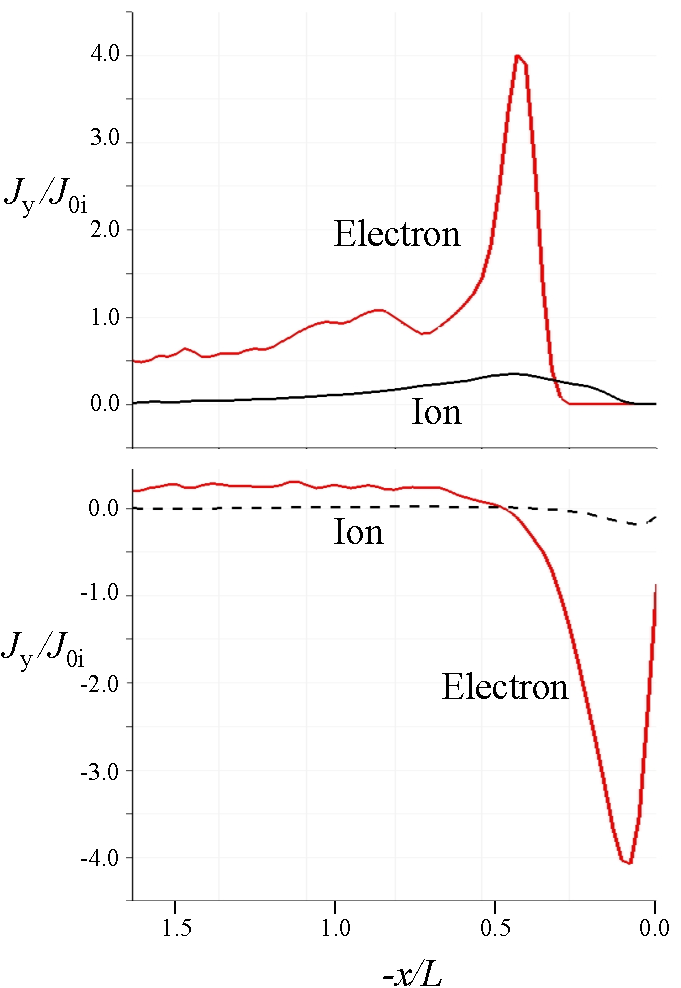
\includegraphics[width=12cm]{./figures/Fig_5_bb-crop.pdf}
\caption{
The $y$ components of the electron and ion current densities are plotted 
along $y/L=z/L=0$ and $y/L=0, z/L=1.0$ in the upper and lower panels, respectively.
The current density is normalized to the ion current density $J_\mathrm{0i}$
in the unperturbed upstream plasma flow.
}
\label{fig:5}
\end{figure}

To examine the boundary layer current in detail, 
we decompose the current into electron and ion components,  
as shown in Figure \ref{fig:5}. 
The upper and lower panels show the $y$ component 
of the current intensity as 
measured along $y/L=z/L=0$ on the magnetic equator 
and $y/L=0, z/L=1.0$ in the +M hemisphere, respectively.
The electron and ion current densities normalized to $J_\mathrm{0i}$ are 
indicated in red and black, respectively. 
As shown in both panels, 
the ion current is much smaller than that of the electrons. 
This implies that the electron current is dominant in the boundary layer.
In the upper panel,
the current has a peak positive value around $x/L=-0.4$. 
We note that because electrons have a negative charge, the 
electron flux points in the negative $y$ direction, which is 
from the R-hand to the L-hand hemisphere. 
On the other hand, in the lower panel, 
the current has a peak negative value at around $x/L=-0.1$, 
which is close to the lunar surface. 
In this case, the direction of the electron flux is toward the R-hand hemisphere.  
As can be seen in both panels of Figure \ref{fig:5}, 
the boundary layer is dominated by the electron current, 
and the electron flux is
toward the L-hand hemisphere at the magnetic equator, while
it is toward the R-hand hemisphere at high latitudes, such as 
around $z/L =1.0$ in the +M hemisphere.
These signatures of the electron flux agree with the
turn-around current structure seen in the three-dimensional space 
shown in Figure \ref{fig:4}.
To understand the structure of the boundary layer current, 
we now consider the electron flux in different planes.

%%---  For Fig 6 and 7, we need to modify the contour maps --

%% - Figure 6-
\begin{figure}[h]
\centering
\noindent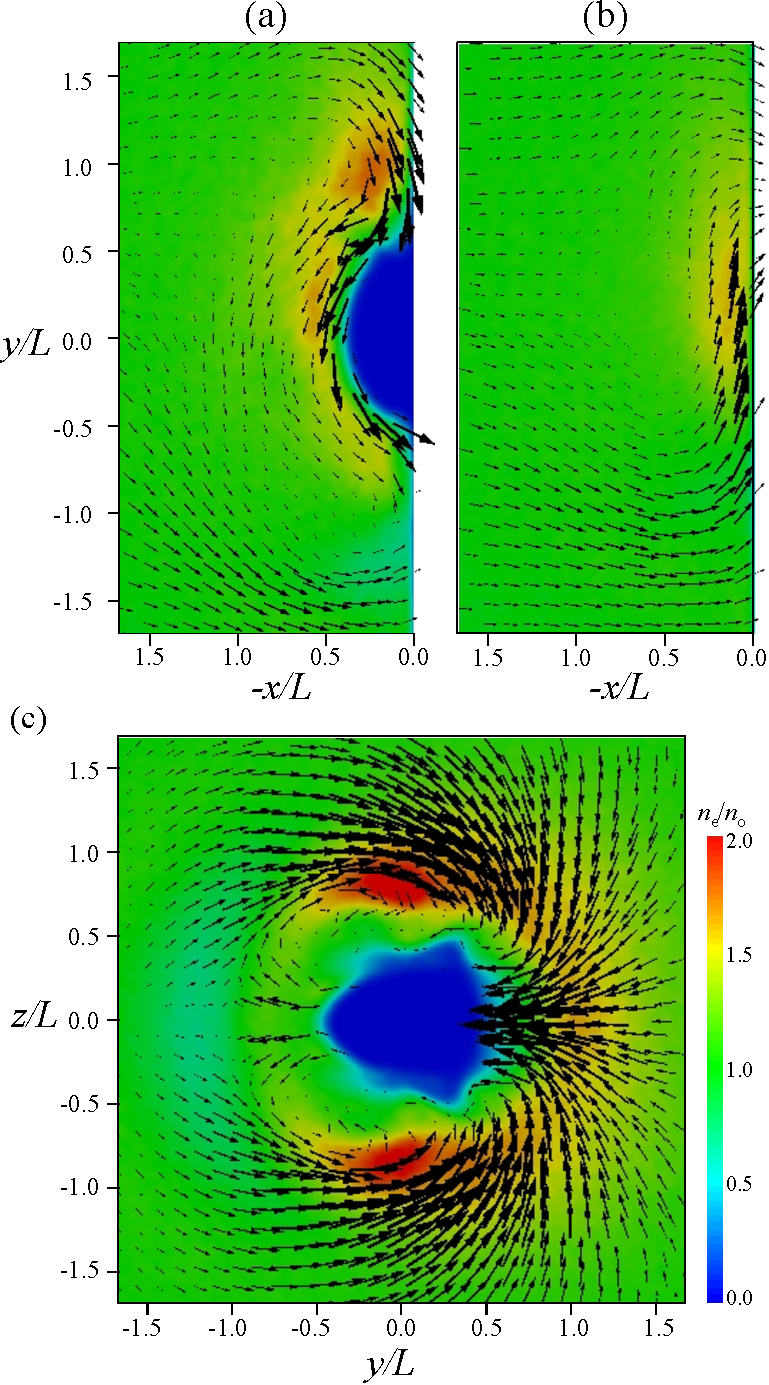
\includegraphics[width=10.5cm]{./figures/Fig_6_bb-crop.pdf}
\caption{
Vectors of electron flux superimposed on the contour map 
of the electron density in the planes of (a) $z/L=0$, (b) $z/L=1.0$, and (c) $x/L=0.1$.
The vectors are normalized to the ion flux in the unperturbed upstream flow.
For example, in (a), the maximum vector shown at $x/L=0.4, y/L=0.0$
corresponds to a flux that is four times the unperturbed ion flux.
}
\label{fig:6}
\end{figure}

Figure \ref{fig:6} shows vectors of the electron flux in different planes, and these are
normalized to that of an ion in the unperturbed upstream flow.
%
In each panel, the contour map shown beneath the vectors indicates the electron density.
Figures \ref{fig:6} (a) and (b) show the profile 
at the magnetic equator $z/L=0$ and at the plane $z/L=1.0$, respectively. 
Note that the direction of the vectors in Figure \ref{fig:6} is
different from that in Figure \ref{fig:4} because 
we show the electron flux, not the electron current.
In Figure \ref{fig:6} (a),  
we see that the electron flux is asymmetric with respect to the line of $y/L=0$.
The electrons enter the R-hand hemisphere  
and then stream along the boundary toward the L-hand hemisphere, creating a region of high electron density along the boundary.
It is interesting that the intense flux is found inside the region of peak density of electrons in the boundary region.
In Figure \ref{fig:6} (b),
we also see a region of intense flux close to the lunar surface.
It should be noted that the direction of the flux is the 
opposite of that seen in Figure \ref{fig:6} (a); it points to the R-hand hemisphere.
%This change of the flux direction basically agrees with 
%the total current profile shown in Fig \ref{fig:4}. 

Figure \ref{fig:6} (c) shows the $y-z$ components of the electron flux 
vectors with $x/L=-0.1$, 
superimposed on the electron density contour map of the corresponding plane.
The panel corresponds to a cross-section of the mini-magnetosphere, 
parallel to the lunar surface.
The contour map indicates an asymmetric density cavity 
surrounded by a high-density boundary layer which is also asymmetric.
These asymmetric density profiles were also discussed in previous studies
(\cite{Deca2014}).
As shown in Figure \ref{fig:6} (c),
a large convective structure of electron flux is found 
in the high-density region of the +M and -M hemispheres.
%
% the following statement is overlapped 
%
%The direction of the electron flux is to the R-hand hemisphere in the +M hemisphere and
%the flux turns around to the low latitude near the magnetic equator $z=0$
%and converges to the R-hand hemisphere.
%Then the flux streams into the magnetic equator toward the direction of 
%the L-hand hemisphere.
The electron flux shown in Figure \ref{fig:6} (c) seems to turn 
in the clockwise direction in the +M hemisphere and the 
counterclockwise direction in the -M hemisphere, the opposite of what was seen for the current vectors in Figure \ref{fig:4}.
%
Although not shown in Figure \ref{fig:6} (c), 
the electron flux converging to the magnetic equator in
the R-hand hemisphere flows along the inner edge of the boundary layer, 
as shown in Figure \ref{fig:6} (a).
The flux profiles shown in Figures \ref{fig:6} (a), (b), and (c) indicate 
that electrons flowing 
to the boundary layer in the +M hemisphere of the mini-magnetosphere
curve toward the R-hand hemisphere 
near the lunar surface and converge to the magnetic equator region; 
the flow then changes direction and moves toward the L-hand magnetosphere
along the inner boundary layer at the magnetic equator.
Electrons flowing to the -M hemisphere show the
same behavior as in the +M hemisphere.
This three-dimensional profile of the electron flux in in basic agreement 
with the all-sky view of the current density vectors 
shown in Figure \ref{fig:4}.

%% - Figure 7-
\begin{figure}[h]
\centering
\noindent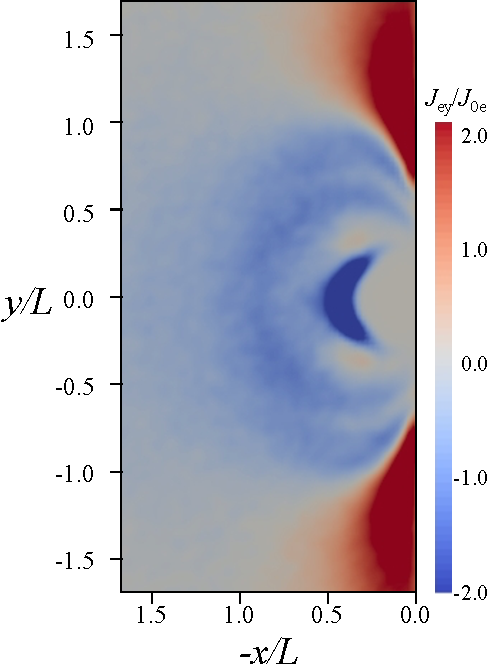
\includegraphics[width=10cm]{./figures/Fig_7_bb-crop.pdf}
\caption{
Contour map of the $y$ component of the electron flux 
on the meridian plane $y/L=0$.
The flux is normalized to the ion flux $n_\mathrm{0}v_\mathrm{flow}$
in the unperturbed upstream plasma flow.
Some magnetic field lines are plotted on the contour map as a reference.
}
\label{fig:7} 
\end{figure}

To show the dependency of the direction of the electron flux on the distance
from the magnetic equator, in Figure \ref{fig:7},
we show a contour map for the $y$ component of the electron flux 
in the $y/L=0$ plane.
As shown in the figure, 
positive values, which imply that the electron flux is toward the R-hand hemisphere,
are found in the regions of approximately $|z/L| > 0.6$ near the lunar surface
in both the +M and -M hemispheres.
In other regions, 
negative values are dominant, as shown in blue, 
which implies that the electron flux is mostly toward the L-hand hemisphere. 
The most intense flux is found 
around $x/L=-0.4$ at the magnetic equator.
We can confirm that because the electron flux is in opposite directions 
at different distances from the magnetic equator, this results in the 
turn-around structures seen in both the +M and -M hemispheres, 
as shown in the current vector profiles in Figure \ref{fig:4}.


\section{Discussion}
%% newly added on 2016/10/12
From the electron flux patterns 
in different planes, as discussed in the previous section, 
we can sketch an overall pattern of the boundary layer current 
in a mini-magnetosphere,
as shown in Figure \ref{fig:sketch}.
%% - Figure sketch-
%% added on 2016/10/15 for the request from $2 referee 
%%
\begin{figure}
\centering
\noindent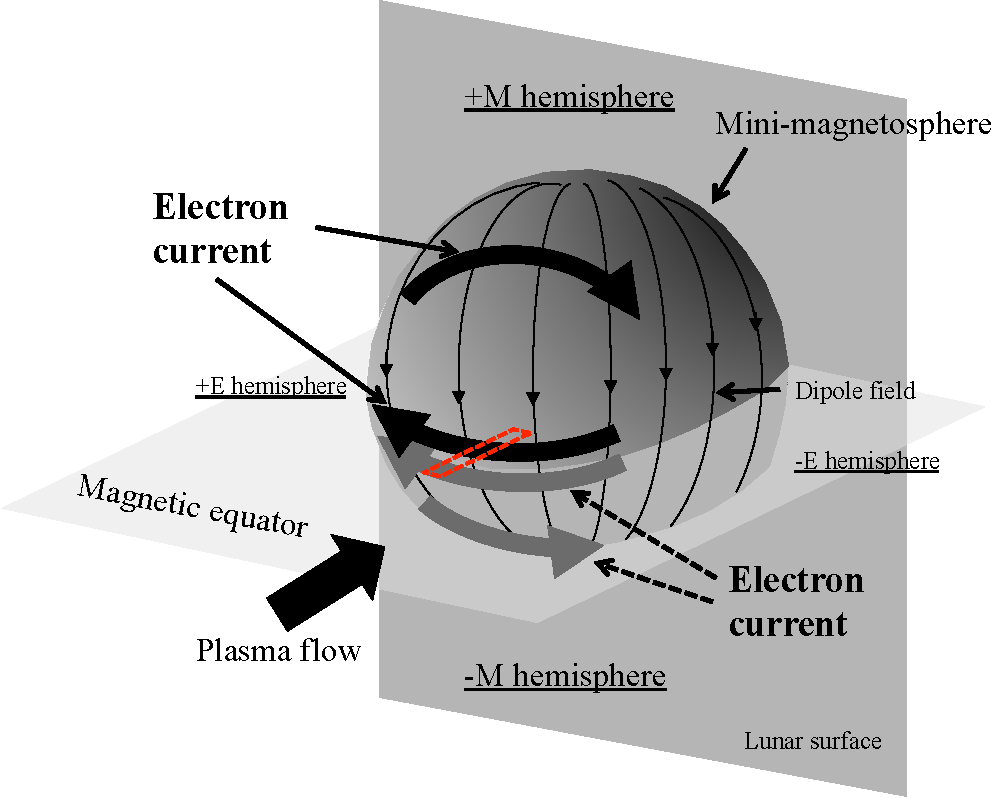
\includegraphics[width=15cm]{./figures/Fig_sketch_bb-crop.pdf}
\caption{
Schematic illustration of the overall pattern of the boundary layer current. 
Symmetric convection of electron current 
is seen in the +M and -M hemispheres. 
}
\label{fig:sketch}
\end{figure}
%
%
A remarkable feature is the major structures 
of turn-around convection of electron current
that are created in the +M and -M hemispheres; these structures are symmetric
with respect to the magnetic equator.
Below, we will present a detailed analysis of the electron motion in the boundary layer in the small region indicated by the red dashed line in Figure \ref{fig:sketch}.
%% - Figure 8-
\begin{figure}
\centering
\noindent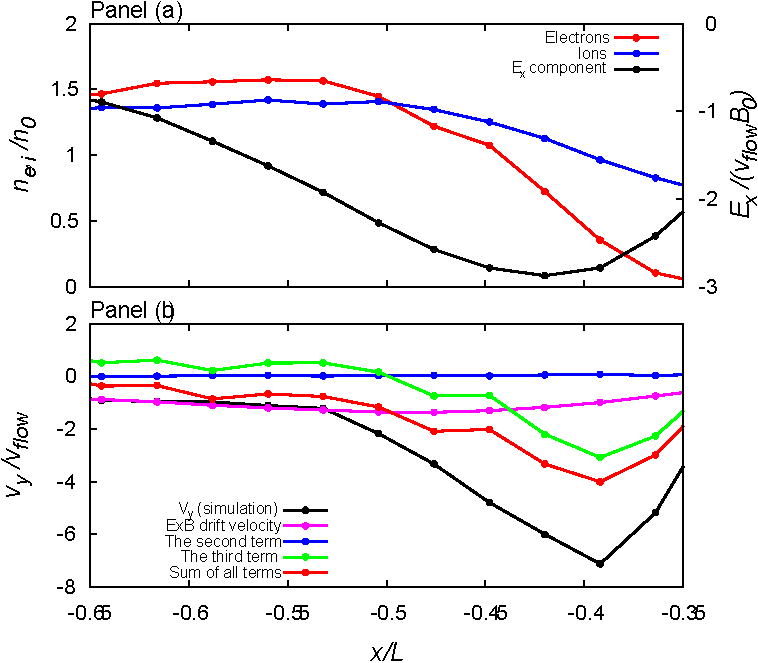
\includegraphics[width=15cm]{./figures/Fig_8_bb-crop.pdf}
\caption{
(a) As obtained in the simulation, electron and ion density variation and $E_x$ intensity 
are plotted in red, blue, and black, respectively, 
along $y/L=z/L=0$ in the region between $x/L = -0.65$ and $-0.35$. 
(b) The theoretical estimate using Equation (\ref{eqn:3}) compared to 
$<v_\mathrm{y-sim}>$, which denotes the average $y$ component of the electron velocity 
of individual electrons in the simulation.
Black, magenta, blue, green, and red curves correspond to $<v_\mathrm{y-sim}>$, $E \times B$ drift velocity obtained with the field values in the simulation, 
the second and terms in Equation (\ref{eqn:3}), and 
$v_\mathrm{y-fld}$ estimated with Equation (\ref{eqn:3}), which corresponds to
the sum of all the terms in the equation.
}
\label{fig:8}
\end{figure}
As shown in the previous section, 
we found that the boundary layer current of the mini-magnetosphere 
mainly consists of the electron flux from the R-hand to the L-hand hemisphere,
as shown in Figure \ref{fig:7}. 
When $r_\mathrm{eL}$ is much smaller than the structure of the
mini-magnetosphere, as in the present case,
the electron flux perpendicular to the dipole field is 
generally considered to be due to electron drift.
In the following discussion, we will consider the electron dynamics in the boundary layer
region surrounded by
the red dashed line in Figure \ref{fig:sketch}.

In Figure \ref{fig:8} (a),
we show one-dimensional plots of the $x$ component of 
the electric field $E_x$ and
electron and ion densities measured along the line $y/L=z/L=0$. 
$E_x$ and the densities are normalized to 
$v_\mathrm{flow} B_\mathrm{0}$ and $n_\mathrm{0}$, respectively.
These quantities are plotted in the region from $x/L = -0.65L$ to $-0.35L$,
Corresponding to the inner boundary layer,
where the plasma density starts decreasing toward the lunar surface.
As shown in black in Figure \ref{fig:8} (a), 
$E_x$ has large negative values, with a peak near $x/L = -0.42 $.
This intense electric field is caused by the difference in density of electrons and ions in the boundary layer.
In particular, between $x/L = -0.5$  and $-0.35$, 
the electron density (shown in red) decreases, and 
the ion density (shown in blue) becomes dominant.
Since ions are less magnetized than electrons in the dipole field region, 
ions can approach the lunar surface closer than can the electrons. 
The resulting $E_\mathrm{x}$ above the magnetic anomaly points in the sunward direction.
Note that the dipole magnetic field points
toward the -M hemisphere and is perpendicular to the magnetic equator, and thus
the $\mbox{\boldmath $E$} \times \mbox{\boldmath $B$}$ velocity
is from the R-hand to the L-hand hemisphere. 
%which corresponds to the direction 
%from the right-hand to the left-hand hemisphere.

We now consider if the intense electron flux observed at the magnetic equator, as
shown in Figure \ref{fig:7}, can be explained by  
the $\mbox{\boldmath $E$} \times \mbox{\boldmath $B$}$ electron drift. 
We will consider the $v_y$ component of the motion of electrons along the line $y/L=z/L=0$.
We will assume that the electrons located in the boundary layer 
are almost magnetized and that
$r_\mathrm{eL}$ is sufficiently small relative to the
structure of the boundary layer that 
we can use the following fluid equation for the electrons:
 
\begin{linenomath}
 \begin{equation}
%  m_\mathrm{e} n_\mathrm{e} \frac{d \mbox{\boldmath v}}{dt}
%    = q_\mathrm{e} n_\mathrm{e}(\mbox{\boldmath E} +
%      \mbox{\boldmath v} \times \mbox{\boldmath B}) - 
%      \nabla P_\mathrm{e}
%  \mbox{\boldmath $B$}
  m_\mathrm{e} n_\mathrm{e} \frac{d \mbox{\boldmath $v_\mathrm{e}$}}{dt}
    = q_\mathrm{e} n_\mathrm{e}
      (\mbox{\boldmath $E$} +
      \mbox{\boldmath $v_\mathrm{e}$} 
      \times
      \mbox{\boldmath $B$}) - 
      \nabla P_\mathrm{e}
 \label{eqn:1}
 \end{equation}
\end{linenomath}
where $v_\mathrm{e}$ and $P_\mathrm{e}$ denote 
the electron velocity and pressure, respectively.
Note that because of the fluid approximation, Equation (\ref{eqn:1}) does not include the effect of 
the finite Larmor radius of the ECM.
In the above equation, if we assume the steady state, 
$\partial{\boldmath v_\mathrm{e}}/\partial{t} = 0$, 
we obtain the following equation for the $x$ component of
the electron velocity $v_x$:

\begin{linenomath}
 \begin{equation}
  m_\mathrm{e} n_\mathrm{e} v_x \frac{\partial v_x}{\partial x}
%% = q_\mathrm{e} n_\mathrm{e} (E_x + v_y B_z) -  K T_\mathrm{e} \frac{\partial n_\mathrm{e}} {\partial x}
%%    = q_\mathrm{e} n_\mathrm{e} (E_x + v_y B_z) -  \nabla (n_\mathrm{e} K_\mathrm{B} T_\mathrm{e})
%%    = q_\mathrm{e} n_\mathrm{e} (E_x + v_y B_z) -  \nabla P_{e}.
    = q_\mathrm{e} n_\mathrm{e} (E_x + v_y B_z) - 
\frac{\partial P_{\mathrm{e}}}{\partial x}
\label{eqn:2}
\end{equation}
\end{linenomath}
Equation (\ref{eqn:2}) shows the electron forces 
in the $x$ direction, which corresponds to the plasma flow direction 
[\cite{Moritaka2012}].
From this relation, we can obtain the $y$ component of the 
electron velocity $v_y$, as follows (to distinguish this from the simulation result, 
we will denote it by $v_{y-fld}$):

%\begin{linenomath}
% \begin{equation}
%    n_\mathrm{e} K_\mathrm{B} T_\mathrm{e}  = \frac{1}{3} m_\mathrm{e}{v_\mathrm{th}}^2
% \end{equation}
%\end{linenomath}

\begin{linenomath}
 \begin{equation}
  v_{y-fld} = 
   - \frac{E_x}{B_z} 
   + \frac {m_\mathrm{e}}{q_\mathrm{e} B_z}v_x\frac{\partial v_x}{\partial x}
   + \frac{1}{q_\mathrm{e} n_\mathrm{e} B_z}\frac{\partial P_{\mathrm{e}}}{\partial x}
%%   + \frac{1}{q_\mathrm{e} n_\mathrm{e} B_z}\nabla (n_\mathrm{e} \frac{1}{3} m_\mathrm{e}{v_\mathrm{th}}^2)
%        =
%   - \frac{E_x}{B_z} 
%   + \frac {m_\mathrm{e}}{q_\mathrm{e} B_z}v_x\frac{\partial v_x}{\partial x}
%   + \frac{m_\mathrm{e}}{3 q_\mathrm{e} n_\mathrm{e} B_z}(n_\mathrm{e} \nabla {v_\mathrm{th}}^2 
%      + {v_\mathrm{th}^2} \nabla {n_\mathrm{e}})
 \label{eqn:3}
 \end{equation}
\end{linenomath}

% --- modify on 160824 @ Brown -----
In Equation (\ref{eqn:3}), 
the first term is 
the $\mbox{\boldmath $E$} \times \mbox{\boldmath $B$}$ velocity,
the second term is the inertial effect, and the third term is the velocity caused 
by the spatial variation of the plasma pressure. 
By using the simulation data for $B_z$, $E_x$, $n_\mathrm{e}$, 
and $v_x$ obtained at each grid point along $y/L=z/L=0$, 
we can use Equation (\ref{eqn:3}) to estimate $v_{y-fld}$. 
In Figure \ref{fig:8} (b), 
the first, second, and third terms of Equation (\ref{eqn:3}) are plotted 
in magenta, blue, and green, respectively.  
The sum of the three terms, which corresponds to $v_{y-fld}$,
is shown in red. 
% As shown in panel (b) of Figure \ref{fig:8},
The second term, which is the inertial term shown in blue, is negligible 
in comparison with the other terms. 
Thus, $v_{y-fld}$ as estimated with Equation (\ref{eqn:3}) is 
dominated by the first and third terms,
which are 
the $\mbox{\boldmath $E$} \times \mbox{\boldmath $B$}$ drift velocity
and the diamagnetic velocity, respectively. 
For a comparison, 
we plotted the simulation results (in black), which were obtained 
using the average of the $v_y$ component of the individual electrons
located at each $x$ position along $y/L=z/L=0$ and ; we will denote 
these results by $<v_{y-sim}>$. 

In the region between $x/L=-0.65$ and $-0.5$, 
the black, red, and magenta curves are in approximate agreement. 
This implies that $<v_{y-sim}>$ in this region 
is mainly due to 
the $\mbox{\boldmath $E$} \times \mbox{\boldmath $B$}$ drift velocity
(shown in magenta),
and thus it can be estimated with fluid theory. 
The term for the diamagnetic velocity (shown in green) is almost zero 
in this region.  

In the inner boundary layer between $x/L=-0.5$ and $-0.35$, 
however,
$<v_{y-sim}>$ (shown in black) does not match 
$v_{y-fld}$ (shown in red).
%
%
%To examine $v_y$ of electrons in the boundary layer current of the magnetosphere, 
%we show spatial variations of relevant physical quantities in \ref{fig:10} 
%such as the electron and ion densities $n_\mathrm{e}, n_\mathrm{i}$ and the $x$ component of 
%the electric field $E_x$ measured along the line of $y/L= z/L =0$.
%%In the second panel in \ref{fig:9}, 
%%we plot $v_y$ values evaluated in the above fluid equation by using the simulation data. 
%%between $x/L = -0.65$ and $-0.5$ 
%%in the simulation domain.
%Note that the $v_y$ data at $x/L= -0.37$ contains some ambiguity because of insufficient 
%number of electrons.  
In particular, the difference between it and the $\mbox{\boldmath $E$} \times \mbox{\boldmath $B$}$ drift velocity (shown in magenta)
becomes large.
While $<v_{y-sim}>$ (shown in black) decreases,
the $\mbox{\boldmath $E$} \times \mbox{\boldmath $B$}$ drift velocity
(in magenta) maintains almost the same value. 
As shown in Figure \ref{fig:8} (a), the intensity of $E_x$ becomes large 
in the corresponding region, and 
the $\mbox{\boldmath $E$} \times \mbox{\boldmath $B$}$ drift velocity
is also assumed to increase. 
However, simultaneously, the dipole magnetic field becomes intense 
in the same region, and eventually 
the $\mbox{\boldmath $E$} \times \mbox{\boldmath $B$}$ drift velocity
takes almost the same values (shown in magenta).
On the other hand, 
$v_{y-fld}$ (shown in red) shows a tendency similar to that of 
$<v_{y-sim}>$ (in black).
Although these do not match quantitatively,
They are qualitatively the same: $v_y$ begins to decrease 
%in the region between $x/L =-0.5$ and $-0.4$ 
in this region.
Under the fluid approximation, this implies that 
$v_y$ is dominated by the diamagnetic velocity, which is defined by 
the third term in Equation (\ref{eqn:3}),
in the region between $x/L =-0.5$ and $-0.4$, 
where the electron density starts to decrease to zero. 

%-- up here modified on 2016/8/23 at Brown.
%-- from here modified on 2016/8/24 at Brown.
Nevertheless, there still exists a quantitative difference between 
$v_{y-fld}$ (in red) and $<v_{y-sim}>$ (in black),
particularly when they are evaluated in the same region.
%%
%% - Figure 9-
%%
\begin{figure}
\centering
\noindent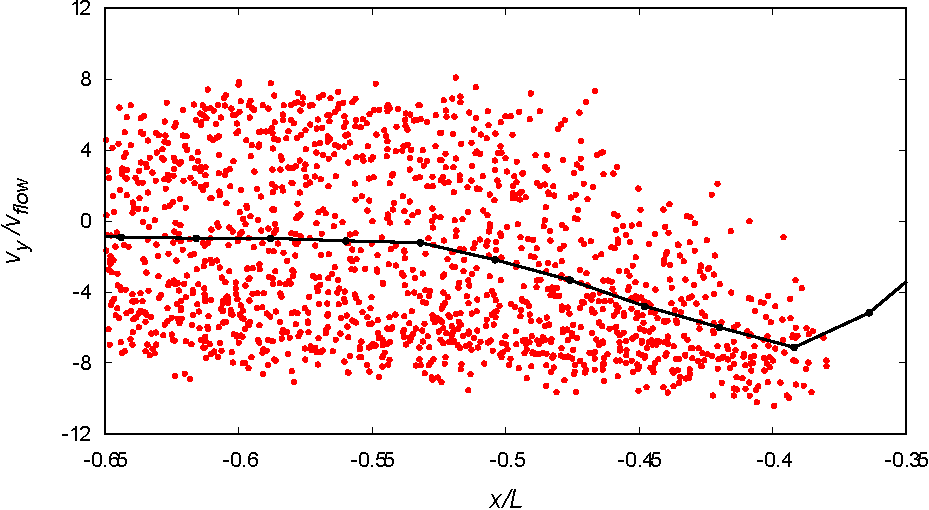
\includegraphics[width=15cm]{./figures/Fig_9_bb-crop.pdf}
\caption{
Electron phase diagram in the $x-v_{y}$ space in the region between $x/L =-0.65$ and $-0.35$,
obtained at the steady state.
The velocity is normalized to $v_\mathrm{flow}$.
}
\label{fig:9}
\end{figure}
In order to understand this difference, 
we consider the finite Larmor radius of the ECM, 
which is evaluated in the PIC simulation. 
%but not considered in Equation (\ref{eqn:3}).
In Figure \ref{fig:9}, 
we plot the $v_y$ component of individual electrons (red dots)
along the line $y/L=z/L=0$.
The velocity values are normalized to $v_\mathrm{flow}$.
As a reference, 
we superimpose the average $v_y$, which is the same as $<v_{y-sim}>$ 
shown in the previous figure.
%  Is this a snapshot ? or time averaged ? -> snapshot at the steady state
%  A question from the #2 referee
%

As is clearly shown, the 
electrons are uniformly distributed 
in the region between $x/L =-0.65$ and $-0.5$.
However, in the region between $x/L =-0.5$ and $-0.4$, 
the velocity distribution starts to converge, 
and the center of the distribution decreases down to 
$v_y/v_{\mathrm{flow}}=-8$. 
It should be noted that 
electrons located in the region between $x/L =-0.65$ and $-0.5$
are distributed on the $v_y$ axis with a velocity range that is much larger 
than $v_{\mathrm{the}}$ of the unperturbed plasma flow. 
The reason for the distribution spread in the $v_{y}$ domain
will be discussed below.
%In the region between $x/L =-0.65$ and $-0.5$,
%$<v_{y-sim}>$ shown in black agrees with the $E times B$ drift velocity as stated above.
%The average $v_y$ shown in black accordingly decreases in this region.
In addition, it is very interesting to note that electrons
in the region between $x/L =-0.5$ and $-0.4$
have no positive $v_y$, which corresponds to movement 
from the L-hand to the R-hand hemisphere.
The above-mentioned features of the electron distribution are closely
associated with the ECM 
and are directly reflected in the curve of $<v_{y-sim}>$ (shown in black).
%We will explain the detail below.
%This phenomenon cannot be predicted with the fluid approximation and can be
%very much associated with ECM around the dipole magnetic field.
%We will explain the detail below.

%%% up here we modified the manuscript on 2/26.

To see the ECM effect on the electron velocity distribution in the boundary layer, 
we plotted individual electrons in the $v_x-v_y$ phase space 
for different regions along $y/L=z/L=0$, as shown in Figure \ref{fig:10}.
Since the dipole magnetic field is perpendicular to the magnetic equator, 
the ECM is directly mapped in the $v_x-v_y$ phase space.
%% - Figure 10-
\begin{figure}
\centering
\noindent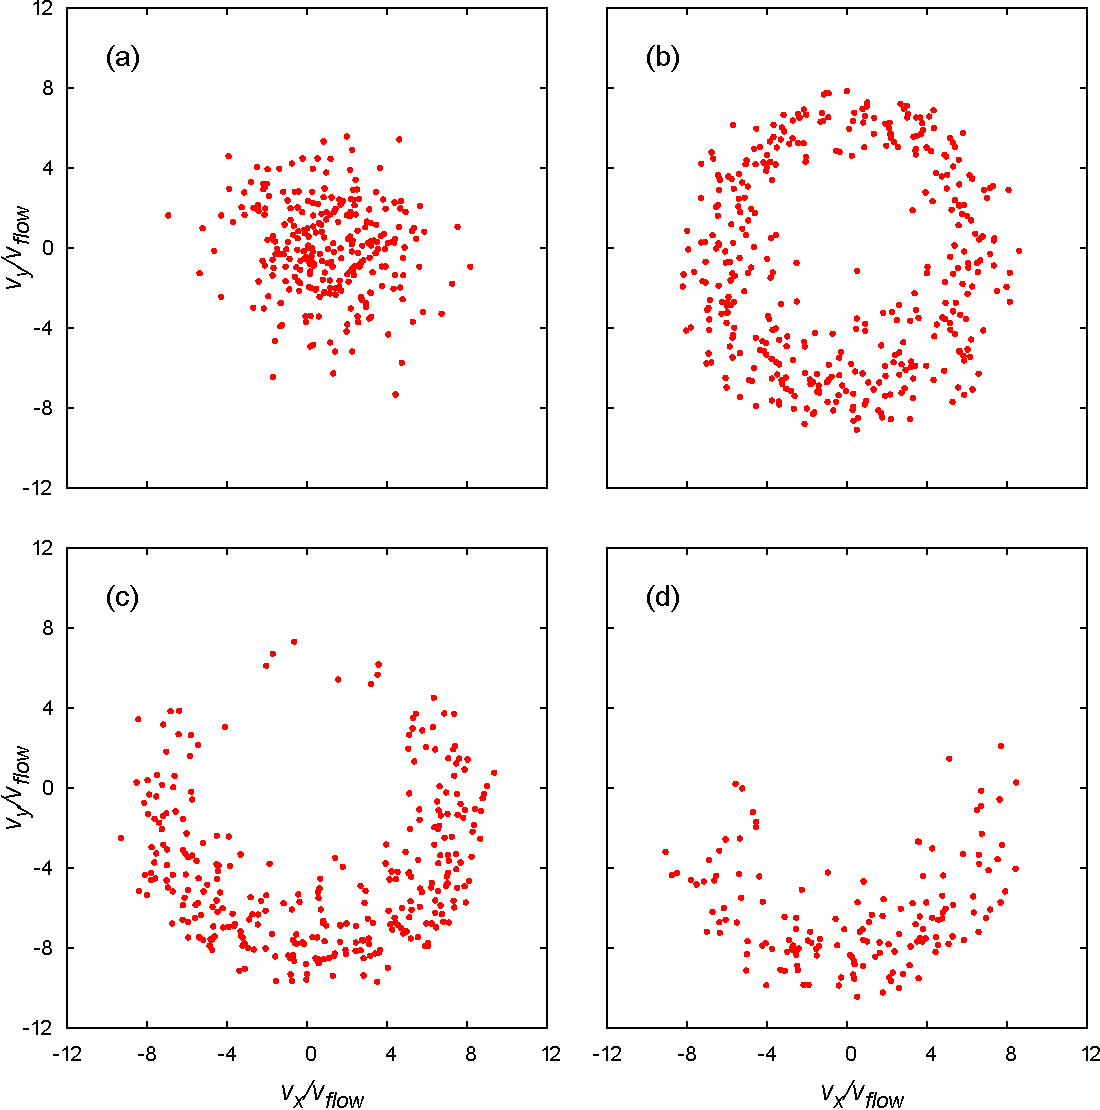
\includegraphics[width=15cm]{./figures/Fig_10_bb-crop.pdf}
\caption{
Electron phase diagrams in the $v_{x}-v_{y}$ space in 
(a) the unperturbed region at $x/L = -5.0$, 
(b) the region between $x/L =-0.59$ and $-0.53$,  
(c) the region between $x/L =-0.48$ and $-0.42$, and
(d) the region between $x/L =-0.42$ and $-0.36$.
}
\label{fig:10}
\end{figure}
Figure \ref{fig:10} (a) shows the region of 
unperturbed plasma flow, while the other panels
show different regions in the boundary layer between $x/L = -0.6$ and -0.4.
Figure \ref{fig:10} (a) shows the unperturbed Maxwellian velocity distribution of the electrons
which have velocity of $v_{\mathrm{flow}}$ in the positive $x$ direction.
It can be seen that the center of the distribution is shifted to the positive $v_x$ direction.
%
When these electrons enter the boundary layer, 
they begin gyrating in the dipole magnetic field and are
affected by the electric field caused by the charge separation
%they start to be accelerated toward the lunar surface 
%by $E_x$ induced by the charge separation, which is 
shown in black in Figure \ref{fig:8} (a).
In Figure \ref{fig:10} (b), we show a phase plot of the electrons located between 
$x/L = -0.59$ and $-0.53$.
It can be clearly seen that the electrons accelerated by $E_x$ form 
a ring-like velocity distribution in the $v_x-v_y$ phase space.
%The electrons which are accelerated toward the negative $x$ direction 
%gain larger velocities and rotate with larger Larmor radius.
The maximum velocity of these electrons is approximately 
$|v|/v_\mathrm{flow} = 8$, which is much larger than 
the ambient thermal velocity $v_{\mathrm{the}}/v_\mathrm{flow} = 2.4$. 
%%as well as the original flow velocity $v_\mathrm{flow}$.
%% Can you explain why v/v_flow = ? 
%% from the referee #2.  2016/10/11
%---
The quantitative analysis of this acceleration of electrons by $E_x$ will be further
discussed below.
%
In Figure \ref{fig:9},
the signature of the electron acceleration
was confirmed in the distribution spread in the region between $x/L =-0.65$ and $-0.5$.
%% - The same sentence above ---
%%Electrons entering the boundary layer
%%are accelerated by $E_x$ and start making the cyclotron motion 
%%with the much larger Larmor radius 
%%around the local magnetic dipole field. 
Figure \ref{fig:10} (c)
shows a phase plot for the electrons located in the boundary layer 
closer to the lunar surface, between $x/L = -0.53$ and $-0.48$, 
where the electron density starts to decrease.
It should be stressed that 
the upper half of the velocity distribution is almost missing in Figure \ref{fig:10} (c).
This nonuniform distribution agrees with the absence of
electrons with positive $v_y$ in
the region $x/L > -0.5$, as shown in Figure \ref{fig:9}.

The reason for this collapse of the ring distribution can be interpreted 
as follows.
%Electrons entering to the boundary layer 
%is basically accelerated toward the lunar surface which is the negative $x$ direction 
%by the electric field induced by the charge separation.
As stated above, the electrons that are accelerated in the boundary layer
gyrate around the local magnetic field with the larger Larmor radius.
Since this process continuously occurs for the electrons 
entering the boundary layer,
the electrons form a gyrotropic ring distribution,
as shown in Figure \ref{fig:10} (b).
%the electron velocity distribution becomes gyrotropic as shown in Panel (b) of \ref{fig:10}.
In this region, 
$<v_{y-sim}>$ agrees well with 
the $\mbox{\boldmath $E$} \times \mbox{\boldmath $B$}$ velocity
because the electrons are gyrotropically 
distributed in the $v_x-v_y$ phase space and the average velocity 
corresponds to that of the guiding center of the ECM corresponding to $<v_{y-sim}>$.
%%This basically agrees with the result obtained in the previous works such as [\cite{Deca2014}].

%--- up to here, I modified in the flight 2016/9/10 
%  need to think the reason why the electron density decreases.


In the inner boundary layer, however, 
we see a quantitative difference between 
$<v_{y-sim}>$ and 
the $\mbox{\boldmath $E$} \times \mbox{\boldmath $B$}$ velocity.
In the region in which $x/L > -0.5$, including the edge of the inner boundary layer, 
the electron density decreases in the antisunward direction 
because the intensity of the local magnetic field becomes large.
%%In this region, 
%%in consideration of the ECM direction,
%%electrons velocity vector points to the direction
%%of the R-hand to the L-hand hemispheres 
%%which corresponds to the negative $v_y$ component 
%%shown in Figure \ref{fig:10}.
Assuming that the Larmor radius of the accelerated electrons
is larger than the region presented in Figure \ref{fig:10} (c), 
electrons in the gyration phase with a positive $v_y$ are 
spatially filtered out of the plot region,
and only the electrons with a negative $v_y$ component
(from the R-hand to the L-hand hemisphere) remain.
%which corresponds to the negative $v_y$ in the phase space.
This is why the electrons with a positive $v_y$ 
are missing in Figure \ref{fig:10} (c).
This filtering due to the finite Larmor radius of the ECM 
causes the maximum $v_y$ value, $|v_y|/v_\mathrm{flow}=8$, to occur  
around $x/L = -0.4$, as
shown in both Figures \ref{fig:9} and \ref{fig:10} (black curves). 

% up here 16/8/25 noon @ brown
To confirm the above discussion of the ECM 
at the inner edge of the boundary layer, in Figure \ref{fig:10} (d),
we show another phase plot, this time of the electrons located between 
$x/L = -0.48$ and $-0.36$.
As shown in the panel, 
most of the electrons have the maximum negative $v_y$ component 
with $|v|/v_\mathrm{flow}=8$. 
This implies that 
due to the finite Larmor radius of the ECM, 
most of the electrons located in the region 
are pointing toward
the L-hand hemisphere. 

Although the intensity of the dipole magnetic field changes depending on 
the distance from the lunar surface, 
the average intensity is approximately $|B|/B_{\mathrm{0}}=20$ 
in the inner boundary layer between $x/L = -0.5$ and $-0.4$.
Assuming that the averaged velocity of the accelerated electrons is 
$|v|/v_\mathrm{flow}=8$, as shown in Figure \ref{fig:10} (d),
we can estimate that $r_\mathrm{eL}$ becomes approximately $0.08L$.
%$ (0.4/1.5)/2.5 =0.1$.
%Then the diameter of the gyrating electrons in the corresponding region roughly becomes around $0.2L$.
This radius is in approximate agreement with the distance 
between $x/L = -0.5$ and -0.4, where
the electron density gradually decreases to zero.

%The spatial width in which the electrons have negative $v_y$ component
%is approximately $0.1L$ which corresponds to the local electron gyroradius.

%%In Figure \ref{fig:8} we showed that at the most inner edge of the magnetosphere
%%there is a gap between the $v_y$ curve of electrons obtained in the simulation
%%and the one estimated with the electron fluid equation. 
%
%

From the above discussion, 
we can conclude that 
the maximum $v_y$ of the electrons, which is found at the inner edge of the 
boundary layer, is not due to the drift of the electron guiding center
but to the ECM velocity, which in turn is due to the acceleration of the local electric field. 
This is one of the most significant findings in this study.
The width of the inner boundary layer with the intense electron flux 
is approximately equivalent to the radius of the local ECM, 
%This means that the width of the boundary layer current 
%is approximately equal to the radius of the local ECM,
which is not related to the ion dynamics.
This is another significant finding of the present study.
%
% Quantitative estimate of the maximum electron velocity
%

We will now quantitatively evaluate the electron acceleration of $|v|/v_\mathrm{flow}=8$, which
is shown in Figure \ref{fig:10}. 
The following is a rough estimate of the electron acceleration in the inner boundary layer.
As we noted previously, 
$E_x$ is enhanced by the charge separation 
in the inner boundary layer and in the sunward direction.
The electrons entering this region are accelerated by this $E_x$.
The kinetic energy gained by these electrons is equal to 
the potential energy created in the corresponding region.
When we focus on the region between $x/L=-0.6$ and $-0.4$ in Figure \ref{fig:8}, 
the average (normalized) value of $E_x$ is roughly -20.
The difference in the electric potential over the region is 
estimated by multiplying the spatial length of the region, 
$0.2 L$, by the average $E_x$.
By using the estimated potential difference, 
we can calculate the kinetic energy which the electrons gain as they travel in this region. 
Note that 
the spatial length of the corresponding region is $0.2 L$, which is about the diameter of 
the electron gyration in the inner boundary layer. 
For simplicity, we can assume that the electrons can be accelerated along the $x$ direction for a distance of $0.2 L$,
without much constraint due to the dipole field.
From the kinetic energy of the electrons calculated above, 
the gained velocity is approximated as $6.3v_\mathrm{flow}$. 
This rough estimate of the electron acceleration in the charge separation region 
is of the same order as the simulation result, which is 
$|v|/v_\mathrm{flow}=8$, as shown in Figures \ref{fig:10} (b) and (c). 

According to the previous studies that have used PIC simulations \citep[e.g.,][]{Deca2014},
the electron current at the mini-magnetosphere boundary is 
simply due to 
the $\mbox{\boldmath $E$} \times \mbox{\boldmath $B$}$ electron drift.
This is true for the macroscopic behavior of electrons in the boundary layer region.
However, 
we found that 
the maximum electron velocity observed at the inner edge of the boundary layer
does not agree with that of the conventional 
$\mbox{\boldmath $E$} \times \mbox{\boldmath $B$}$ drift.
Considering the finite Larmor radius of the ECM, 
we clarified that the maximum velocity of the electrons was 
due to 
%%the spatial filtering caused by the effect of the finite Larmor radius of 
the acceleration by the electric field in the boundary layer.

From a macroscopic point of view, 
a question remains about the closure of the current in the boundary layer.
In the present simulation, 
we assumed no emission of photoelectrons from the lunar surface.
In addition, there exists no ionosphere in the lunar environment.
In such a situation, 
the boundary current of a mini-magnetosphere 
cannot be closed by the plasma that originates at the lunar surface.
Although we have not yet performed a detailed analysis of the current closure in a
lunar surface environment, 
we can imagine that the plasma flux 
at the boundary of the mini-magnetosphere
will eventually impinge on the lunar surface and thus
contribute to the surface charge.

As shown in Figure \ref{fig:2} (c),
we see high-density regions of electrons
at the polar regions around $|z|/L =0.5$ in
the vicinity of the lunar surface.
In these regions,
the magnetic fields converge, and the incoming electrons concentrate
in the cusp-like dipole fields.
Eventually, the electron density becomes higher than that of the ions.
However, it is difficult for the electrons to enter the region
just outside the cusp regions around $|z|/L = 1.0$,
where the dipole field becomes 
almost perpendicular to the plasma flow, 
and so
the density becomes rather small.  
On the other hand, it is easier for
ions in the plasma flow to approach the lunar surface
than it is for electrons, since the ions have relatively large inertia.
The ion density thus becomes high near the lunar surface.
A similar signature 
is found in the charge density profile at the magnetic equator, as shown in Figure \ref{fig:3} (c).
In the boundary layer regions around $|y|/L = 1.0$, where the densities are high 
for both species,
the charge density becomes positive 
because the ion density is higher than that of the electrons.
This occurs because the large $r_\mathrm{iL}$ allows the ions to approach the lunar surface.
Considering these signatures of the charge density, we note that 
the surface charging in the region surrounding the plasma cavity 
of the mini-magnetosphere can be positive
because the dominant contribution is due to ions impinging on the surface.
Since a quantitative analysis of the surface charging is 
beyond the scope of the current study, 
we leave it as an area of future work.

%
% up to here 2016/2/11 holiday around 17:00 at home
%


%% appended on 2016/10/14 for the further discussion for #2 referee
%
In previous studies based on hybrid particle simulation, it has been found that an
electric field in the sunward direction is induced above the magnetic anomaly 
due to the decoupling of electron and ion motion in the boundary layer; this occurs 
even without separation of charge [\cite{Jarvinen2014}  \cite{Fatemi2015}].
%This enhancement of the electric field is also confirmed in the present study 
%in the straightforward manner due to the charge separation, which is also 
%shown in other works such as [\cite{Deca2014}].
In the present simulation, 
the electric field was similarly enhanced in the boundary layer.
From an evaluation of these results, it is clear that
the significant factor for the enhancement of the electric field is
the difference between the motion of electrons and that of ions in the boundary layer;
this was simulated both in the full particle and the hybrid models.
The charge separation observed in the present simulation
was due to the decoupling of the two species of particle in the dipole field. 

A unique and significant aspect of the present study is the use of a full particle model
that allows the analysis of the electron dynamics by solving for the dynamics of the individual particles.
This provides a large advantage over 
the hybrid and MHD simulations.
In particular, as shown in Figures \ref{fig:9} and \ref{fig:10}, a full particle simulation
allows us to obtain the electron velocity distribution, 
the acceleration of the electrons by the electric field, and 
the resulting formation of a ring-like velocity distribution 
in the boundary layer.
These results are new findings  
which have not been previously presented.

In this study, we assumed that $B_{\mathrm{0}}$ was uniform and pointed 
in the positive $z$ direction.
%The static magnetic field in the simulation domain includes 
%$B_{\mathrm{0}}$ and the dipole field of the magnetic anomaly.
%As a result of the interaction by the plasma flow, 
%the dipole field is compressed and deformed. 
%A mini-magnetosphere is eventually created above the magnetic anomaly.
Like the Earth's magnetosphere, 
the orientation of $B_{\mathrm{0}}$ may affect the shape of 
the mini-magnetosphere due to its interaction with the dipole field. 
As an area of future work, the orientation of $B_{\mathrm{0}}$ 
on the physics of the mini-magnetosphere 
%%in terms of its shape and plasma dynamics in the boundary layer 
should be examined.

\section{Conclusions}
We studied the boundary layer current in 
a mini-magnetosphere created above a lunar magnetic anomaly
by performing three-dimensional electromagnetic particle-in-cell simulations.
In this study, we focused on the following two aspects on the
electron current, which dominates in the boundary layer.
The first is the three-dimensional structure of 
the boundary layer current of the mini-magnetosphere. 
The second is the electron cyclotron motion 
in the boundary layer current, examined at the magnetic equator.
The simulations revealed that the profile of 
the electron boundary current shows 
turn-around convection structures 
in the +M and -M hemispheres, and these are symmetric with respect to the magnetic equator.
The electrons flowing to +M and -M hemispheres 
of the mini-magnetosphere
change direction and head toward the R-hand hemisphere 
near the lunar surface; they converge at the magnetic equator. 
The electron flow then changes direction and heads toward the L-hand hemisphere, 
traveling along the inner boundary of the mini-magnetosphere on the magnetic equator.
The simulations also revealed the mechanism by which the electrons obtain their maximum velocity, which is
observed at the edge of the inner boundary layer,
where the electron density gradually decreases to zero.
We clarified that the maximum electron velocity
is due to the acceleration by the electric field, which is
enhanced by the charge separation, and it is 
not simply due to the $\mbox{\boldmath $E$} \times \mbox{\boldmath $B$}$ drift.
For the ECM, we clarified that 
the maximum velocity of electrons, which is also observed 
at the edge of the inner boundary layer, is due to 
the spatial filtering caused by 
the effect of the finite Larmor radius of the electrons 
accelerated by the electric field.
We also confirmed that the width of the boundary current layer 
is approximately equal to the radius of the local ECM
These simulation results strongly suggest that the 
ECM and the finite Larmor radius of the electrons are significant 
for understanding the electron current in the boundary layer of a mini-magnetosphere. 

As an area of future work, 
we plan to further study the electron flux in the boundary layer 
near the polar regions, where the flux direction is opposite 
that observed at the magnetic equator.
Unlike the situation at the magnetic equator, in the polar regions,
the direction of the dipole field is not simply 
perpendicular to the plasma flow. 
%If the electron flux is also dominated by the $E \times B$ drift, 
Thus, when
the $\mbox{\boldmath $E$} \times \mbox{\boldmath $B$}$ drift 
is a major source of electron flux, it is necessary to consider the relative angle between
the local $E$-field due to the charge separation and 
the dipole magnetic field.
It is also necessary to consider the finite Larmor radius 
of the electron in order to examine the electron velocity 
at the edges of the boundary current in the polar regions.

%%%%%%%%%%%%%%%%%%%%%%%%%%%%%%%%
%% Optional Appendix goes here
%
% \appendix resets counters and redefines section heads
% but doesn't print anything.
% After typing \appendix
%
%\section{Here Is Appendix Title}
% will show
% Appendix A: Here Is Appendix Title
%
%%%%%%%%%%%%%%%%%%%%%%%%%%%%%%%%%%%%%%%%%%%%%%%%%%%%%%%%%%%%%%%%
%
% Optional Glossary or Notation section, goes here
%
%%%%%%%%%%%%%%
% Glossary is only allowed in Reviews of Geophysics
% \section*{Glossary}
% \paragraph{Term}
% Term Definition here
%
%%%%%%%%%%%%%%
% Notation -- End each entry with a period.
% \begin{notation}
% Term & definition.\\
% Second term & second definition.\\
% \end{notation}
%%%%%%%%%%%%%%%%%%%%%%%%%%%%%%%%%%%%%%%%%%%%%%%%%%%%%%%%%%%%%%%%
%
%  ACKNOWLEDGMENTS

\begin{acknowledgments}
This work was supported by JSPS KAKENHI Grant Numbers 23340148 and 16H04058. 
Computation resources have been provided by the KDK of Kyoto University
and the Pi-computer  of ECCSE in Kobe University.
The data for this paper are available on request; 
contact H.~Usui at h-usui@port.kobe-u.ac.jp.
\end{acknowledgments}

%% ------------------------------------------------------------------------ %%
%%  REFERENCE LIST AND TEXT CITATIONS
%
% Either type in your references using
% \begin{thebibliography}{}
% \bibitem{}
% Text
% \end{thebibliography}
%
% Or,
%
% If you use BiBTeX for your references, please use the agufull08.bst file (available at % ftp://ftp.agu.org/journals/latex/journals/Manuscript-Preparation/) to produce your .bbl
% file and copy the contents into your paper here.
%
% Follow these steps:
% 1. Run LaTeX on your LaTeX file.
%
% 2. Make sure the bibliography style appears as \bibliographystyle{agufull08}. Run BiBTeX on your LaTeX
% file.
%
% 3. Open the new .bbl file containing the reference list and
%   copy all the contents into your LaTeX file here.
%
% 4. Comment out the old \bibliographystyle and \bibliography commands.
%
% 5. Run LaTeX on your new file before submitting.
%
% AGU does not want a .bib or a .bbl file. Please copy in the contents of your .bbl file here.

\bibliographystyle{agufull08}
%\bibliography{luna_151002}
\bibliography{luna_161005}

%%\begin{thebibliography}{}
%\providecommand{\natexlab}[1]{#1}
%\expandafter\ifx\csname urlstyle\endcsname\relax
%  \providecommand{\doi}[1]{doi:\discretionary{}{}{}#1}\else
%  \providecommand{\doi}{doi:\discretionary{}{}{}\begingroup
%  \urlstyle{rm}\Url}\fi
%
%\bibitem[{\textit{Atkinson and Sloan}(1991)}]{AtkinsonSloan}
%Atkinson, K., and I.~Sloan (1991), The numerical solution of first-kind
%  logarithmic-kernel integral equations on smooth open arcs, \textit{Math.
%  Comp.}, \textit{56}(193), 119--139.
%
%\bibitem[{\textit{Colton and Kress}(1983)}]{ColtonKress1}
%Colton, D., and R.~Kress (1983), \textit{Integral Equation Methods in
%  Scattering Theory}, John Wiley, New York.
%
%\bibitem[{\textit{Hsiao et~al.}(1991)\textit{Hsiao, Stephan, and
%  Wendland}}]{StephanHsiao}
%Hsiao, G.~C., E.~P. Stephan, and W.~L. Wendland (1991), On the {D}irichlet
%  problem in elasticity for a domain exterior to an arc, \textit{J. Comput.
%  Appl. Math.}, \textit{34}(1), 1--19.
%
%\bibitem[{\textit{Lu and Ando}(2012)}]{LuAndo}
%Lu, P., and M.~Ando (2012), Difference of scattering geometrical optics
%  components and line integrals of currents in modified edge representation,
%  \textit{Radio Sci.}, \textit{47},  RS3007, \doi{10.1029/2011RS004899}.

%%\end{thebibliography}

%Reference citation examples:

%...as shown by \textit{Kilby} [2008].
%...as shown by {\textit  {Lewin}} [1976], {\textit  {Carson}} [1986], {\textit  {Bartholdy and Billi}} [2002], and {\textit  {Rinaldi}} [2003].
%...has been shown [\textit{Kilby et al.}, 2008].
%...has been shown [{\textit  {Lewin}}, 1976; {\textit  {Carson}}, 1986; {\textit  {Bartholdy and Billi}}, 2002; {\textit  {Rinaldi}}, 2003].
%...has been shown [e.g., {\textit  {Lewin}}, 1976; {\textit  {Carson}}, 1986; {\textit  {Bartholdy and Billi}}, 2002; {\textit  {Rinaldi}}, 2003].

%...as shown by \citet{jskilby}.
%...as shown by \citet{lewin76}, \citet{carson86}, \citet{bartoldy02}, and \citet{rinaldi03}.
%...has been shown \citep{jskilbye}.
%...has been shown \citep{lewin76,carson86,bartoldy02,rinaldi03}.
%...has been shown \citep [e.g.,][]{lewin76,carson86,bartoldy02,rinaldi03}.
%
% Please use ONLY \citet and \citep for reference citations.
% DO NOT use other cite commands (e.g., \cite, \citeyear, \nocite, \citealp, etc.).

%% ------------------------------------------------------------------------ %%
%
%  END ARTICLE
%
%% ------------------------------------------------------------------------ %%
\end{article}
%
%
%% Enter Figures and Tables here:
%
% DO NOT USE \psfrag or \subfigure commands.
%
% Figure captions go below the figure.
% Table titles go above tables; all other caption information
%  should be placed in footnotes below the table.
%
%----------------
% EXAMPLE FIGURE
%
 %\begin{figure}
 %\noindent\includegraphics[width=20pc]{samplefigure.eps}
 %\caption{Caption text here}
 %\label{figure_label}
 %\end{figure}
%
% ---------------
% EXAMPLE TABLE
%
%\begin{table}
%\caption{Time of the Transition Between Phase 1 and Phase 2\tablenotemark{a}}
%\centering
%\begin{tabular}{l c}
%\hline
% Run  & Time (min)  \\
%\hline
%  $l1$  & 260   \\
%  $l2$  & 300   \\
%  $l3$  & 340   \\
%  $h1$  & 270   \\
%  $h2$  & 250   \\
%  $h3$  & 380   \\
%  $r1$  & 370   \\
%  $r2$  & 390   \\
%\hline
%\end{tabular}
%\tablenotetext{a}{Footnote text here.}
%\end{table}



%%%%%%%%%%%%%%%%%%%%%%%%%%%%%%%%
%% Optional Appendix goes here
%
% \appendix resets counters and redefines section heads
% See below for how to make sideways figures or tables.

\end{document}













